    
\begin{figure}[h]
  \centering
%    \subfigure[]{\includegraphics[width=0.45\textwidth]{figures/SRdefinition/kineMap/GG_symQQC1_x12_nJet30.pdf}}
    \subfigure[]{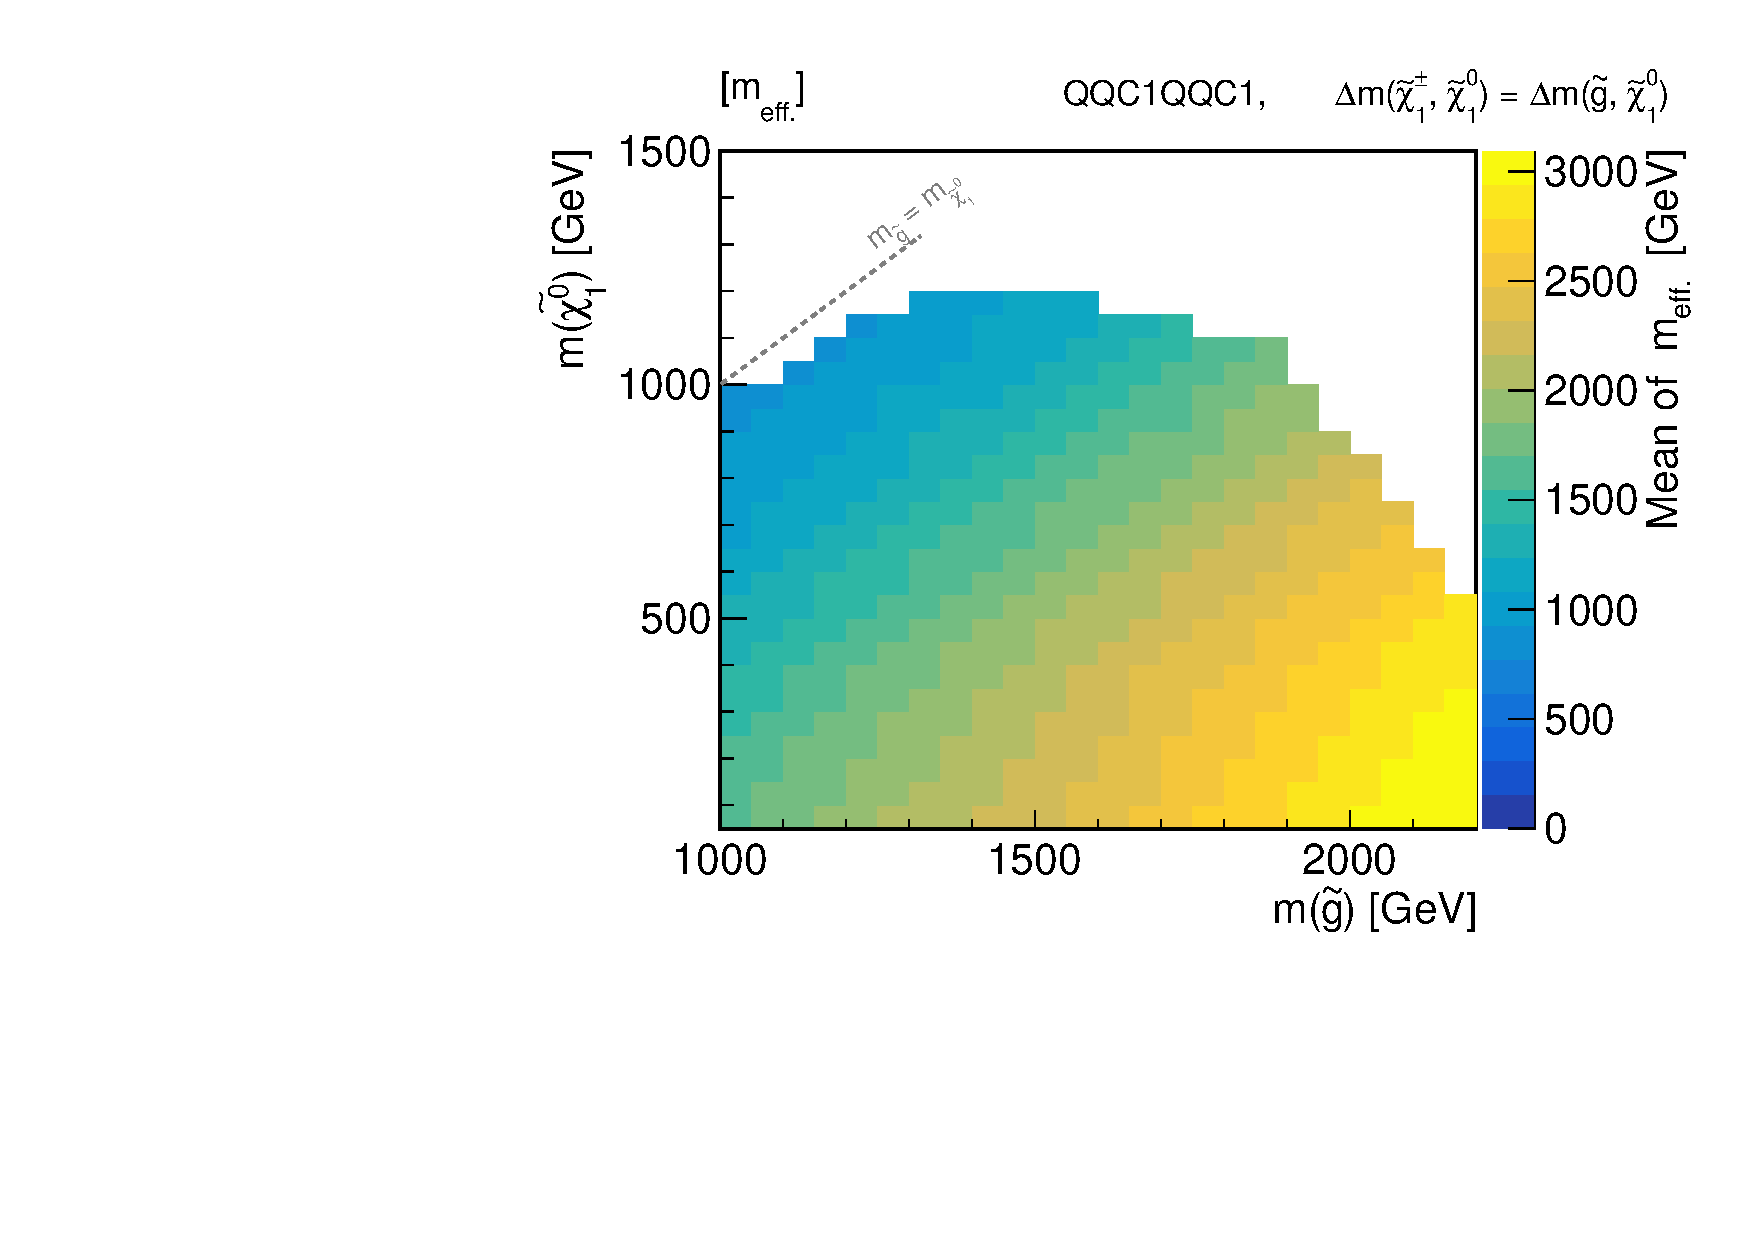
\includegraphics[width=0.45\textwidth]{figures/SRdefinition/kineMap/GG_symQQC1_x12_meff.pdf}}
    \subfigure[]{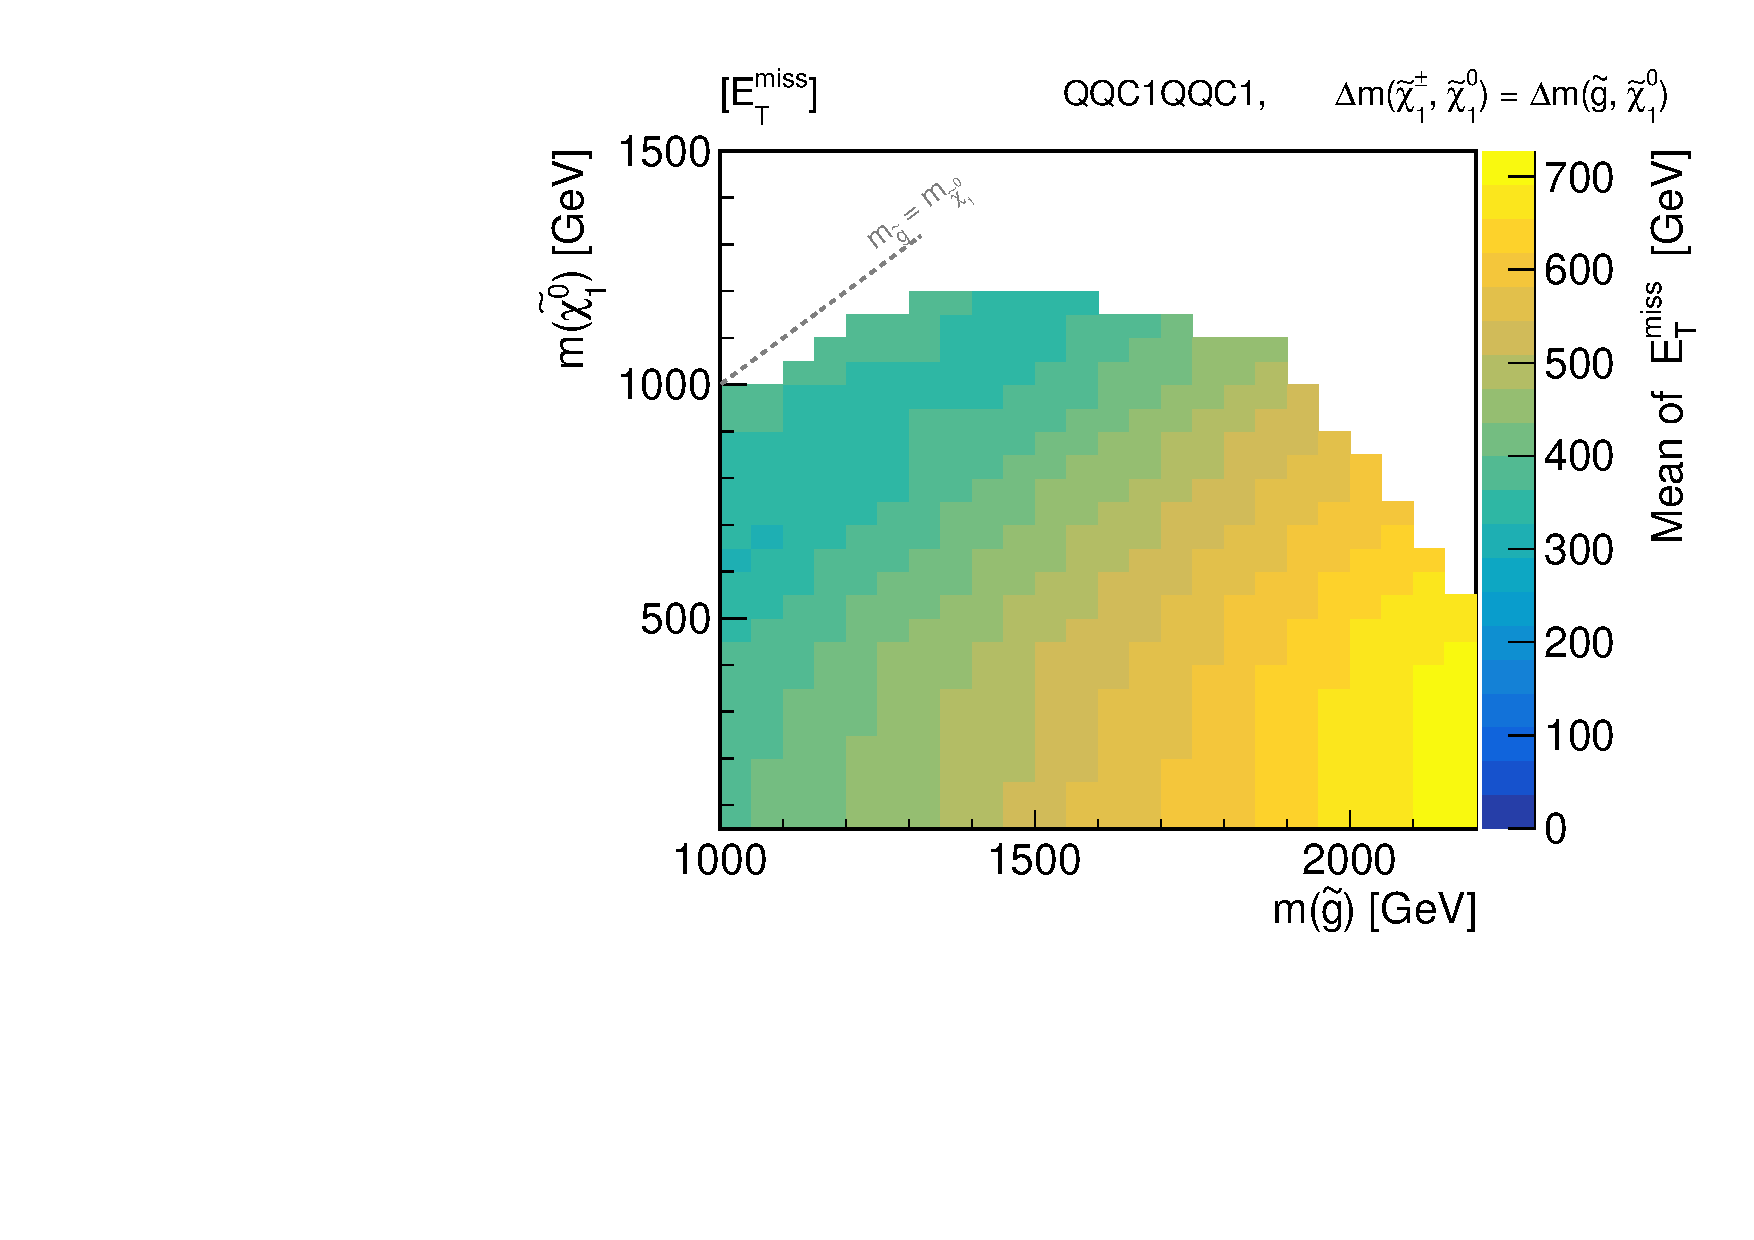
\includegraphics[width=0.45\textwidth]{figures/SRdefinition/kineMap/GG_symQQC1_x12_met.pdf}}
    \subfigure[]{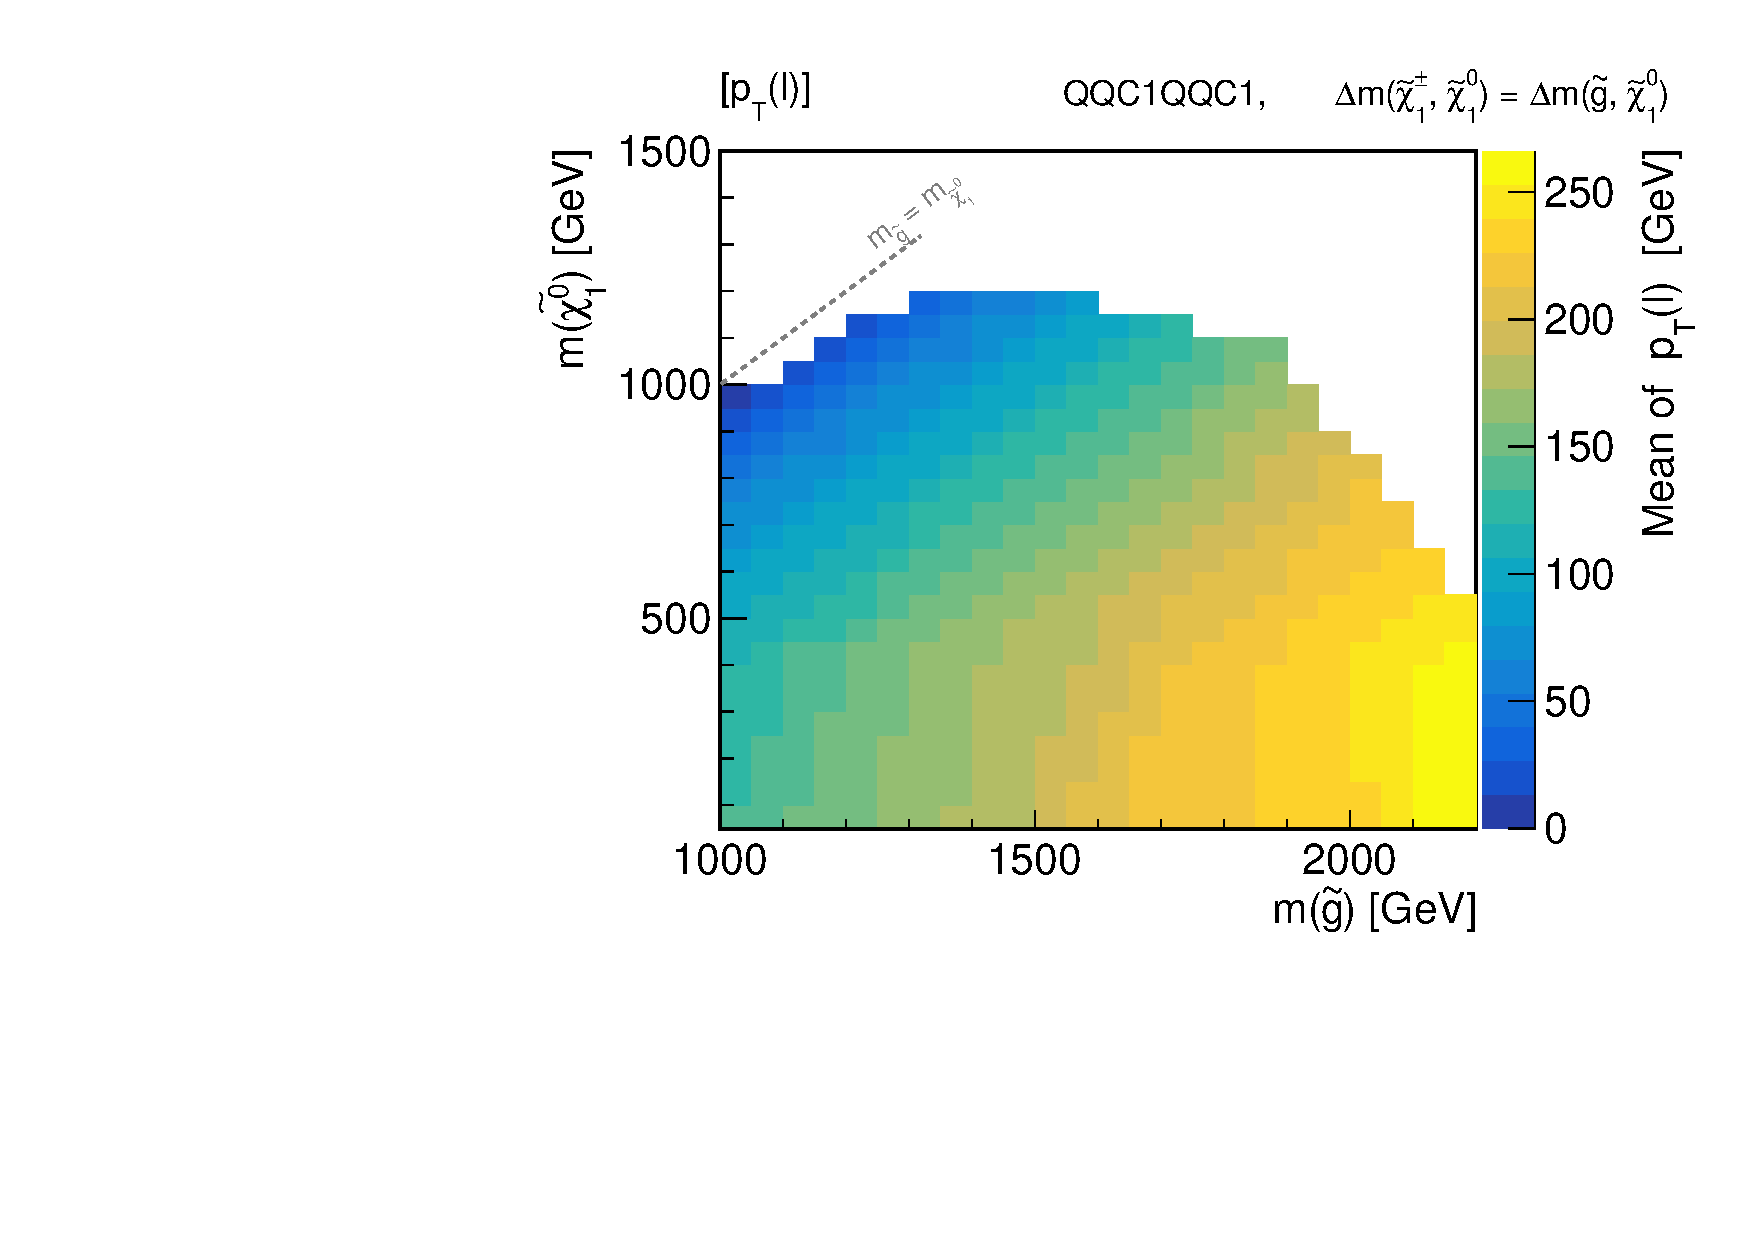
\includegraphics[width=0.45\textwidth]{figures/SRdefinition/kineMap/GG_symQQC1_x12_lep1Pt.pdf}}
    \subfigure[]{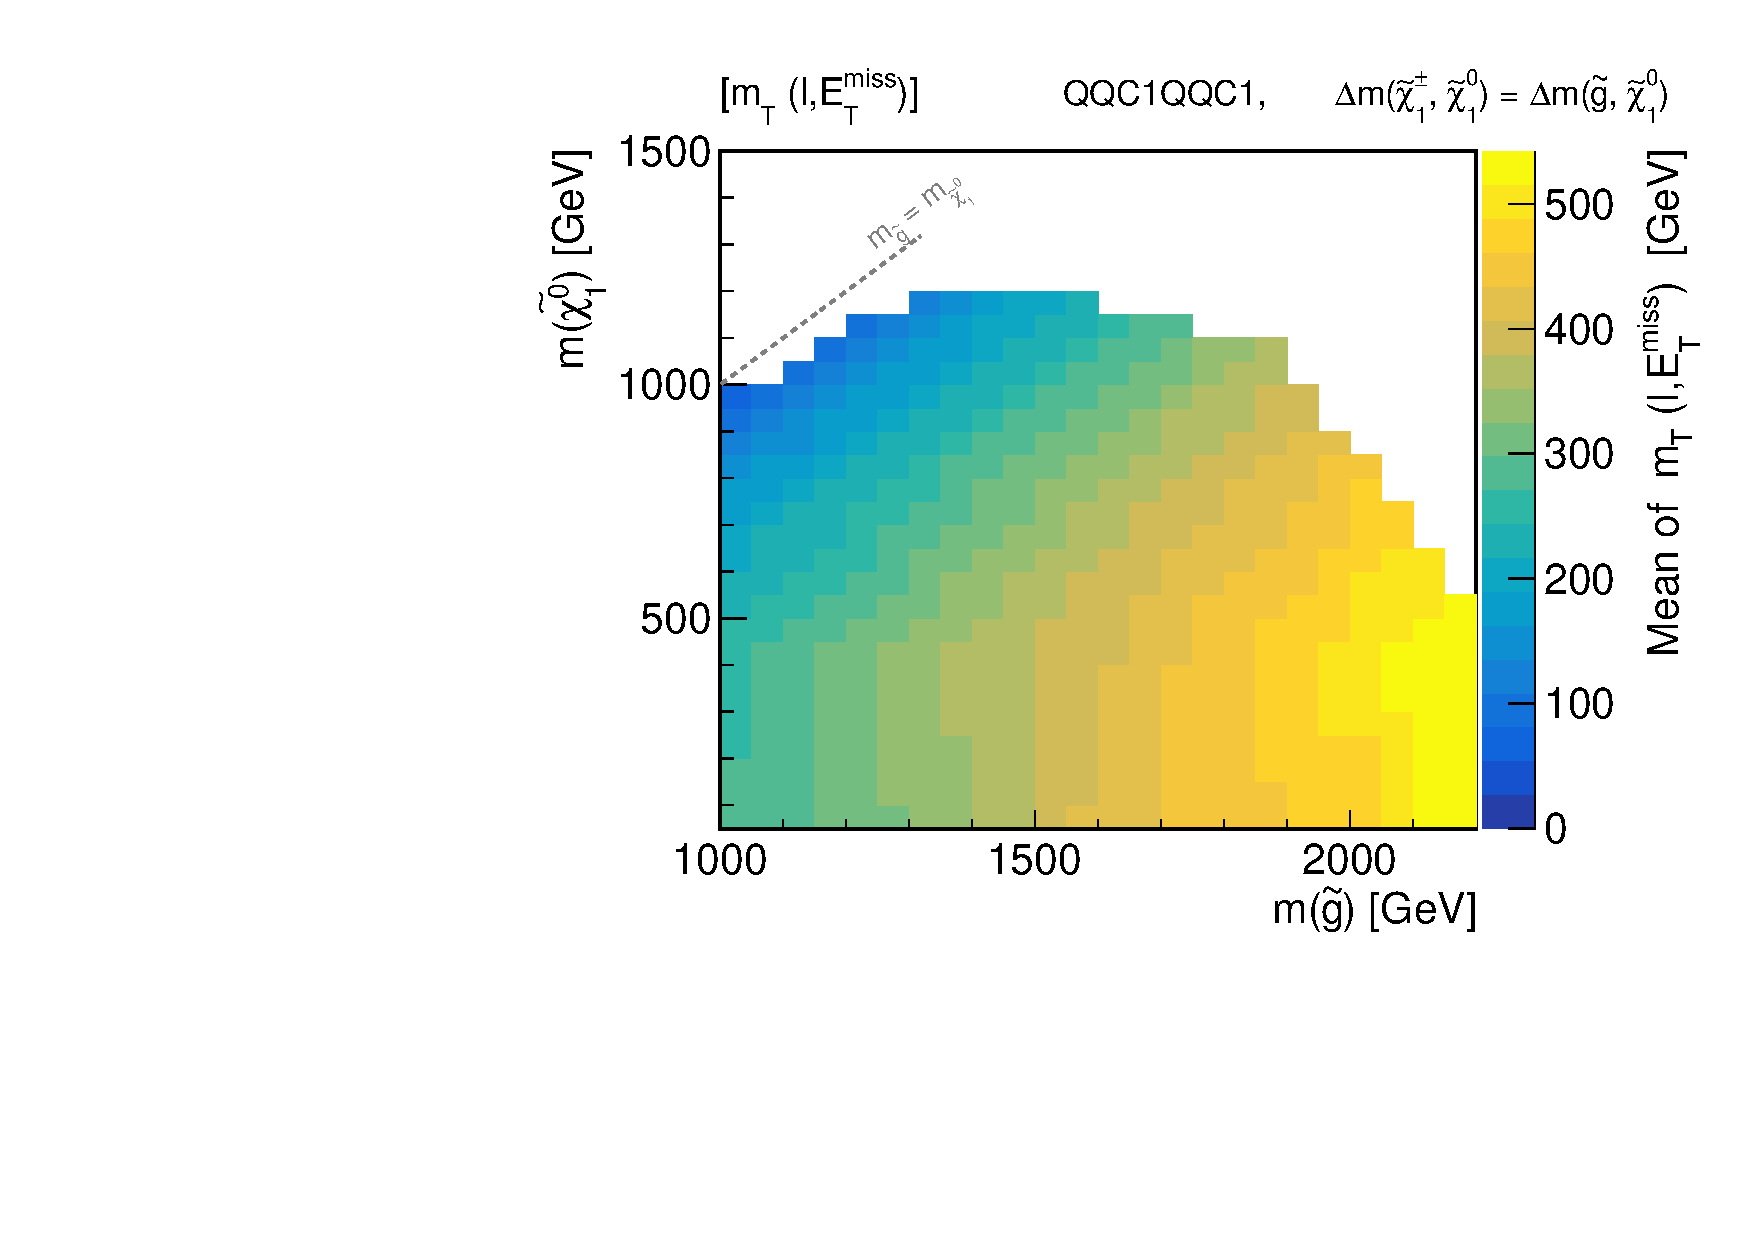
\includegraphics[width=0.45\textwidth]{figures/SRdefinition/kineMap/GG_symQQC1_x12_mt.pdf}}
    \subfigure[]{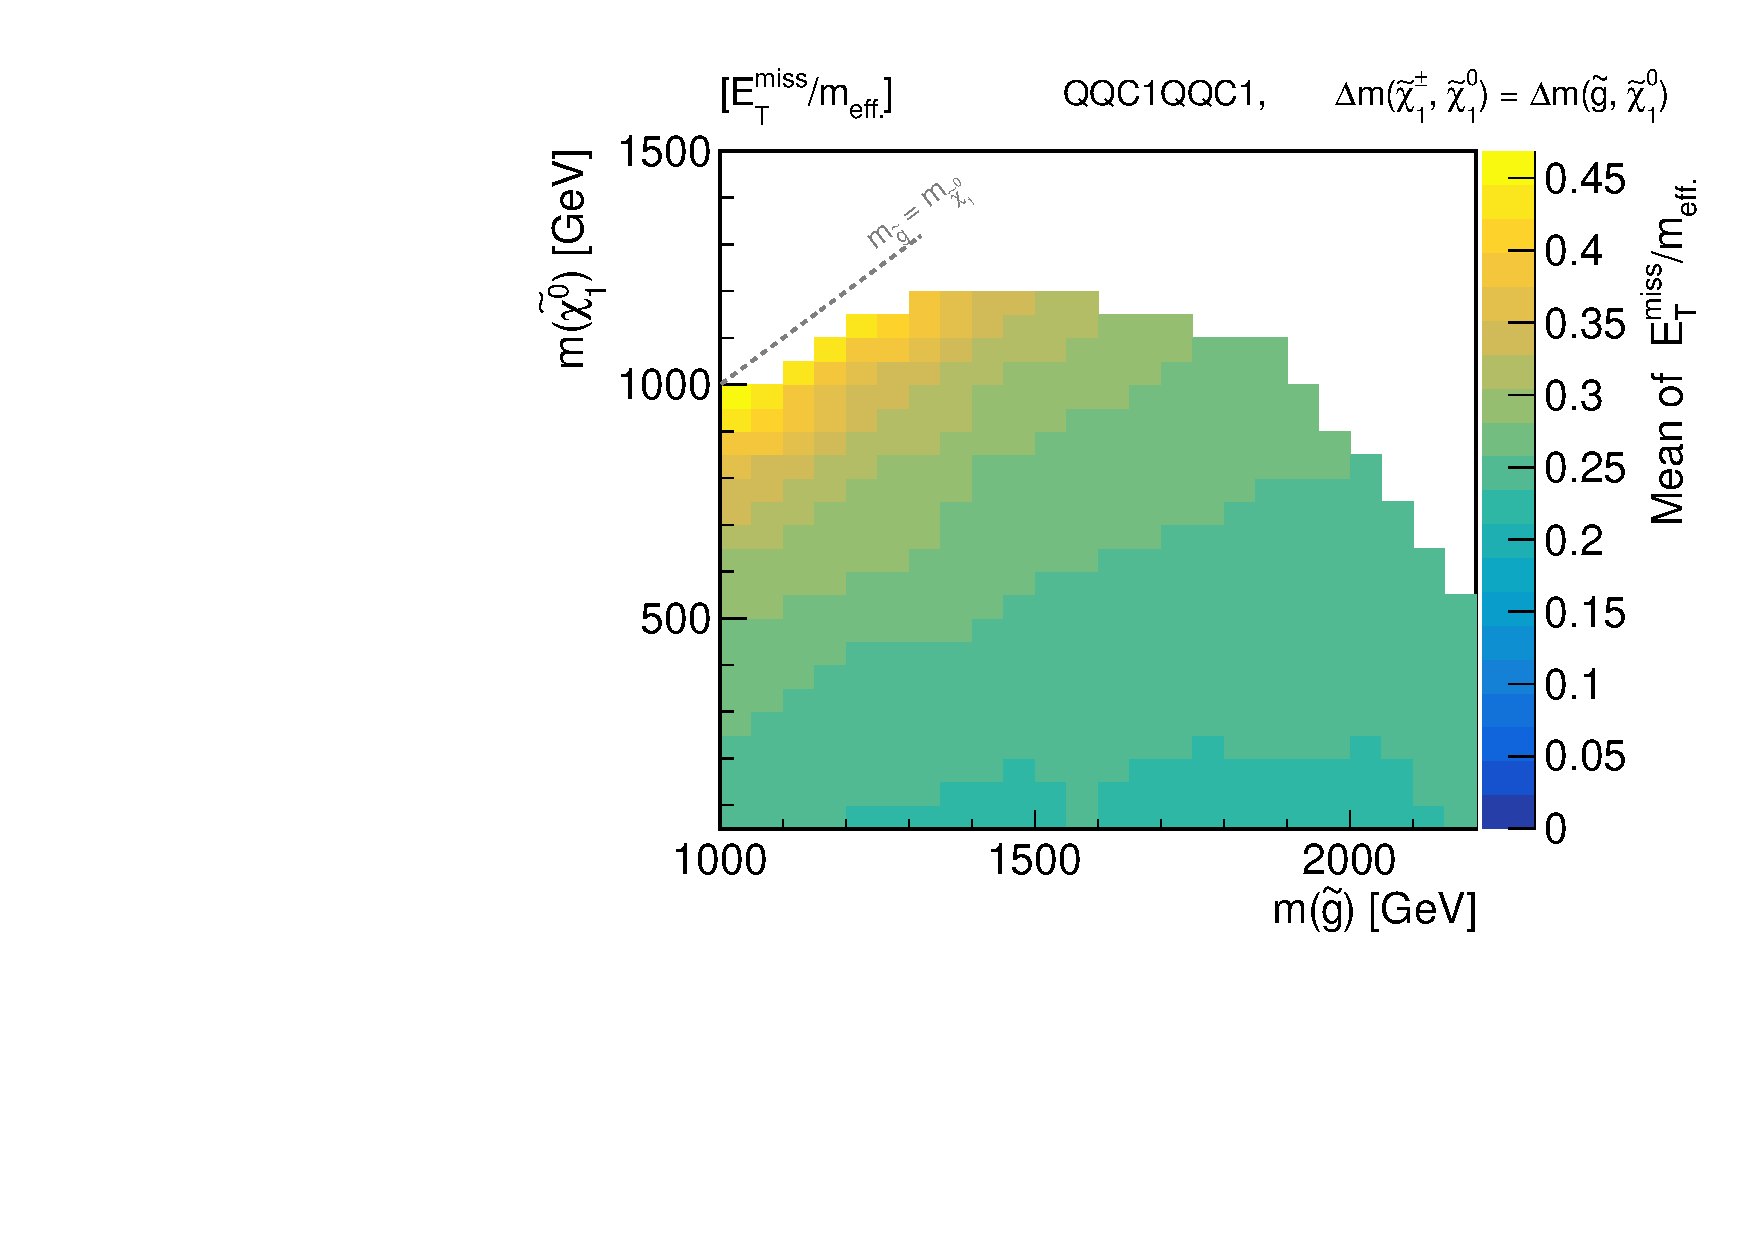
\includegraphics[width=0.45\textwidth]{figures/SRdefinition/kineMap/GG_symQQC1_x12_metOverMeff.pdf}}
    \subfigure[]{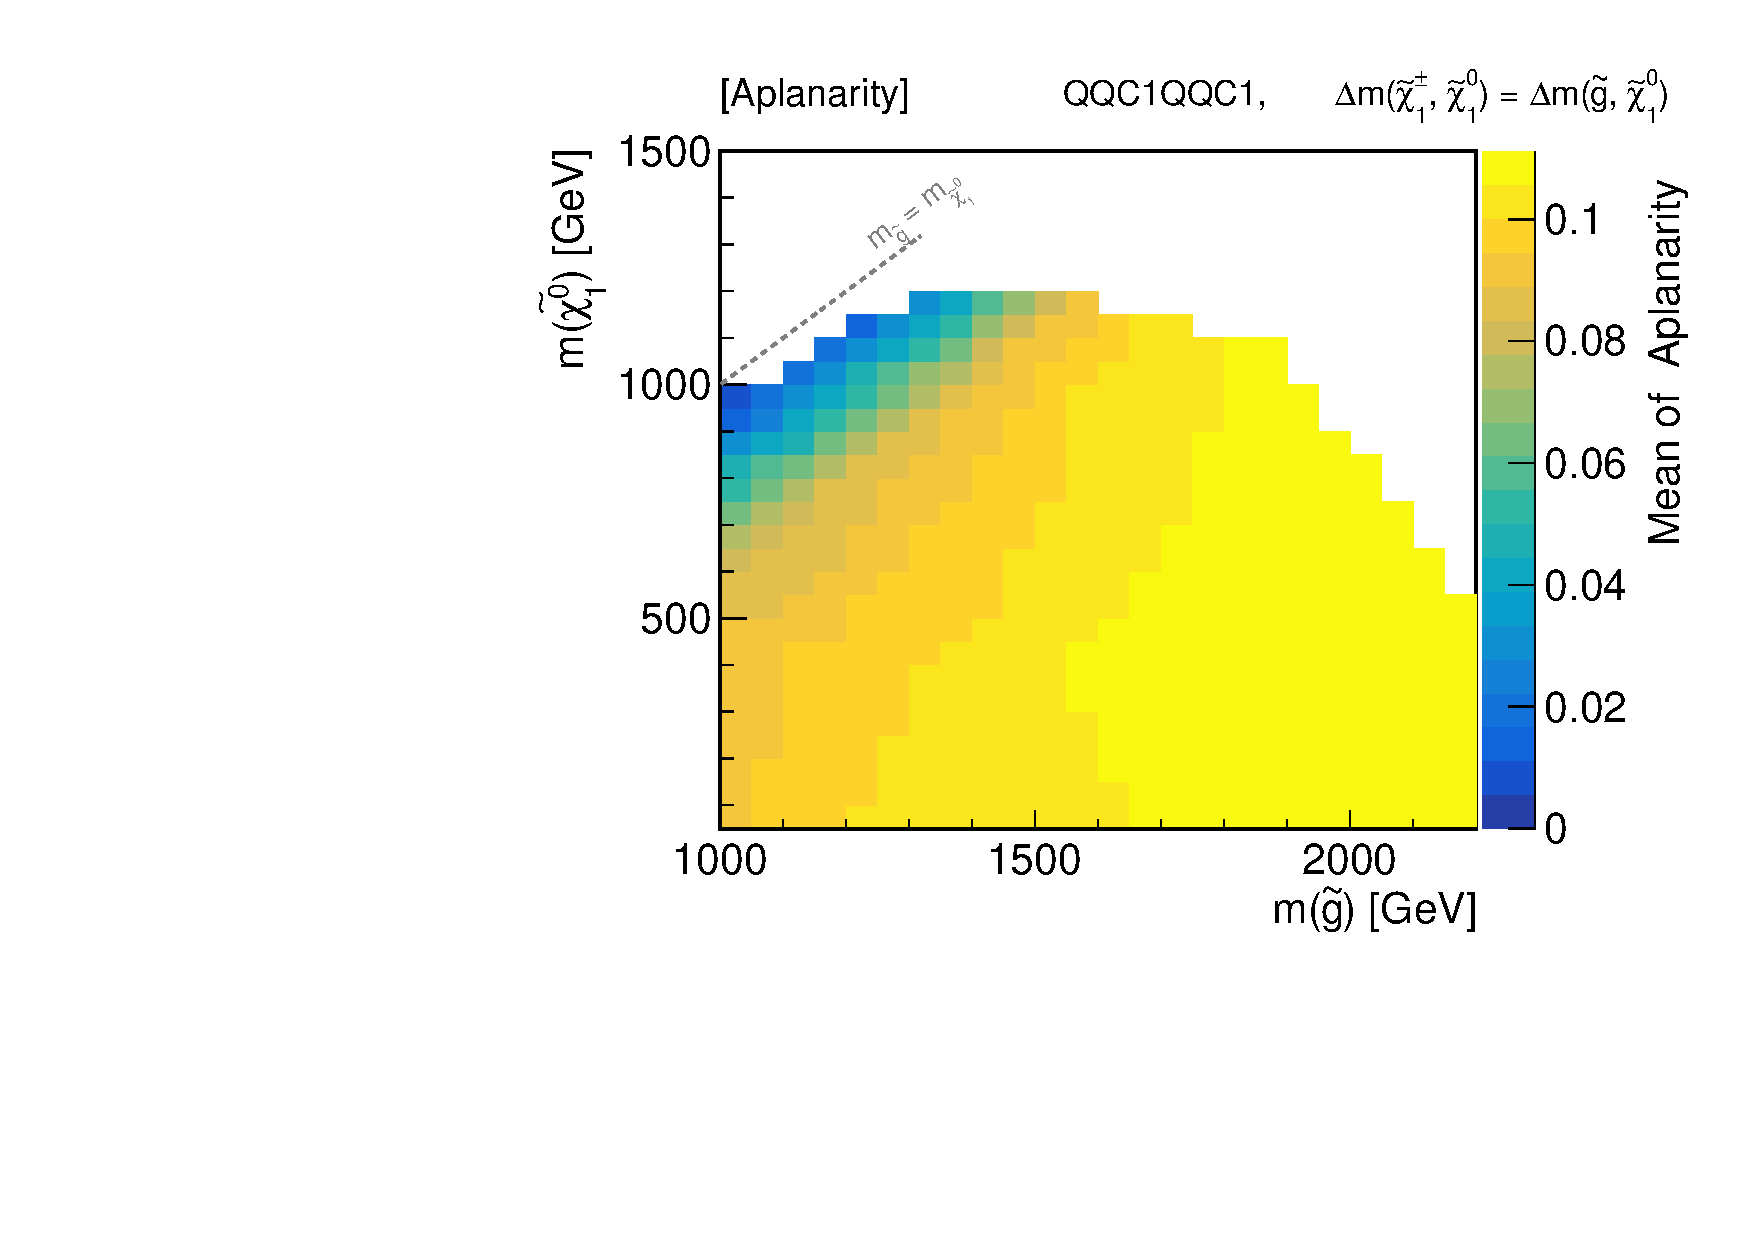
\includegraphics[width=0.45\textwidth]{figures/SRdefinition/kineMap/GG_symQQC1_x12_LepAplanarity.pdf}}
    \caption{ Mean of (a) $\meffInc$ (b) $\met$ (c) $\lepPt$ (d) $\mt$ (e) $\metOverMeff$ (f) aplanarity, for the QQC1QQC1 \xhalf grid, after the pre-selection. 
      \label{fig::SRdefinition::kineMap_QQC1QQC1_x12} 
    }
\end{figure}
 

\begin{figure}[h]
  \centering
%    \subfigure[]{\includegraphics[width=0.45\textwidth]{figures/SRdefinition/kineMap/GG_symQQC1_varx_nJet30.pdf}}
    \subfigure[]{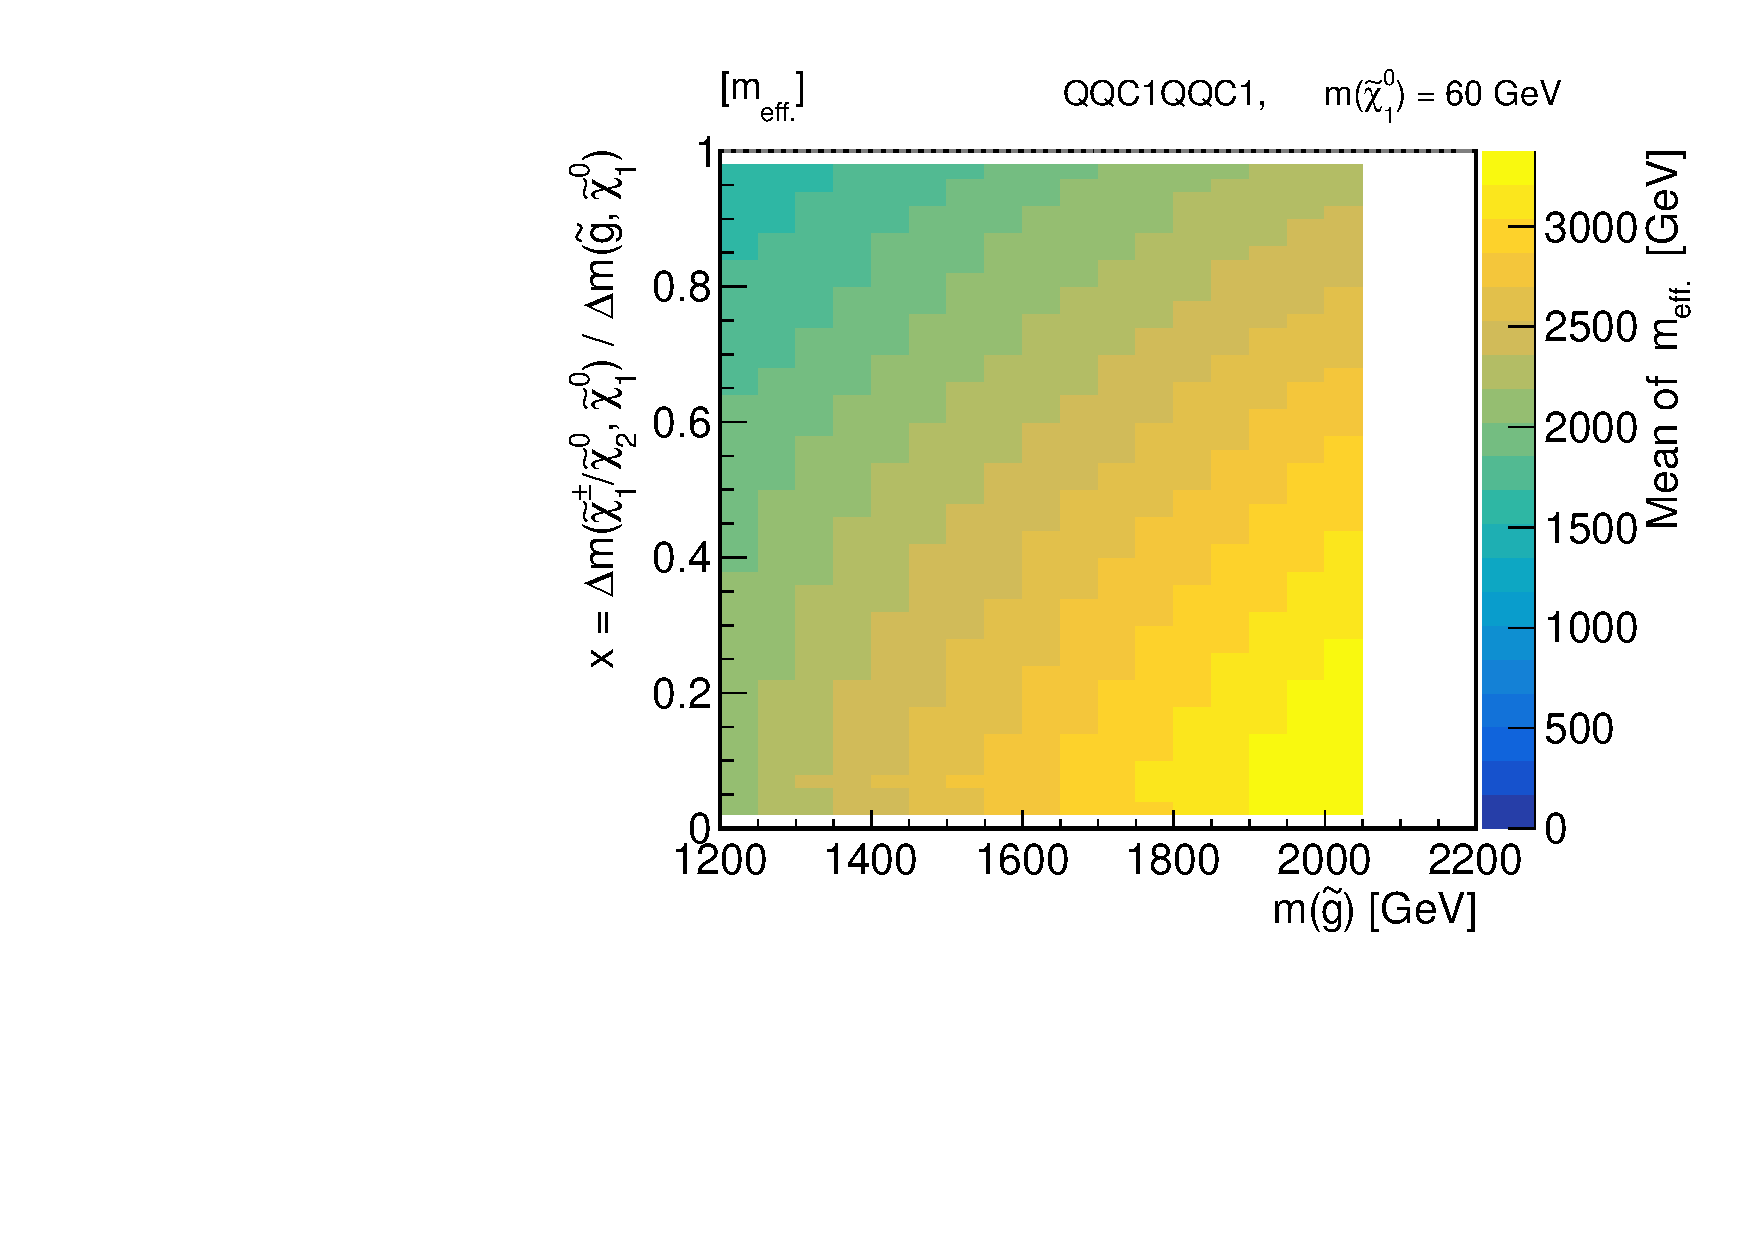
\includegraphics[width=0.45\textwidth]{figures/SRdefinition/kineMap/GG_symQQC1_varx_meff.pdf}}
    \subfigure[]{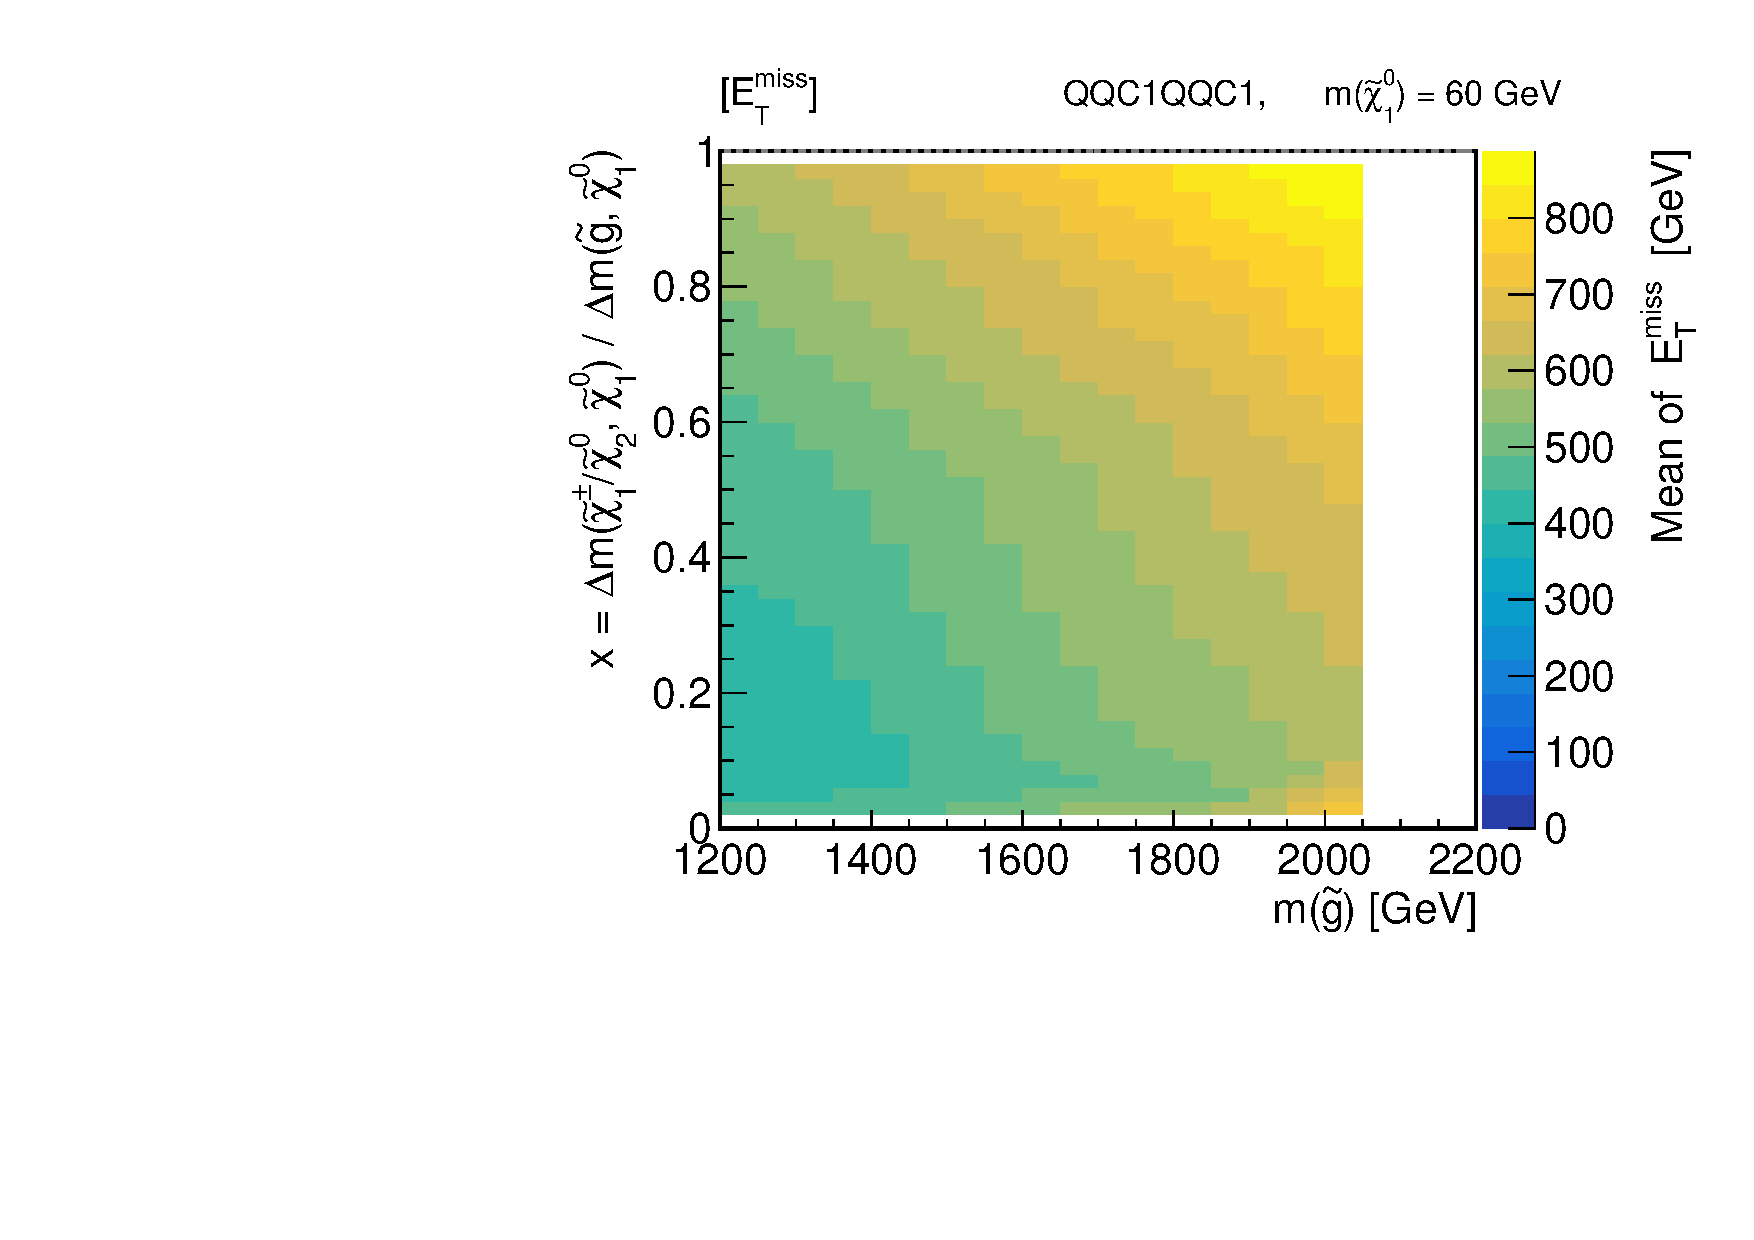
\includegraphics[width=0.45\textwidth]{figures/SRdefinition/kineMap/GG_symQQC1_varx_met.pdf}}
    \subfigure[]{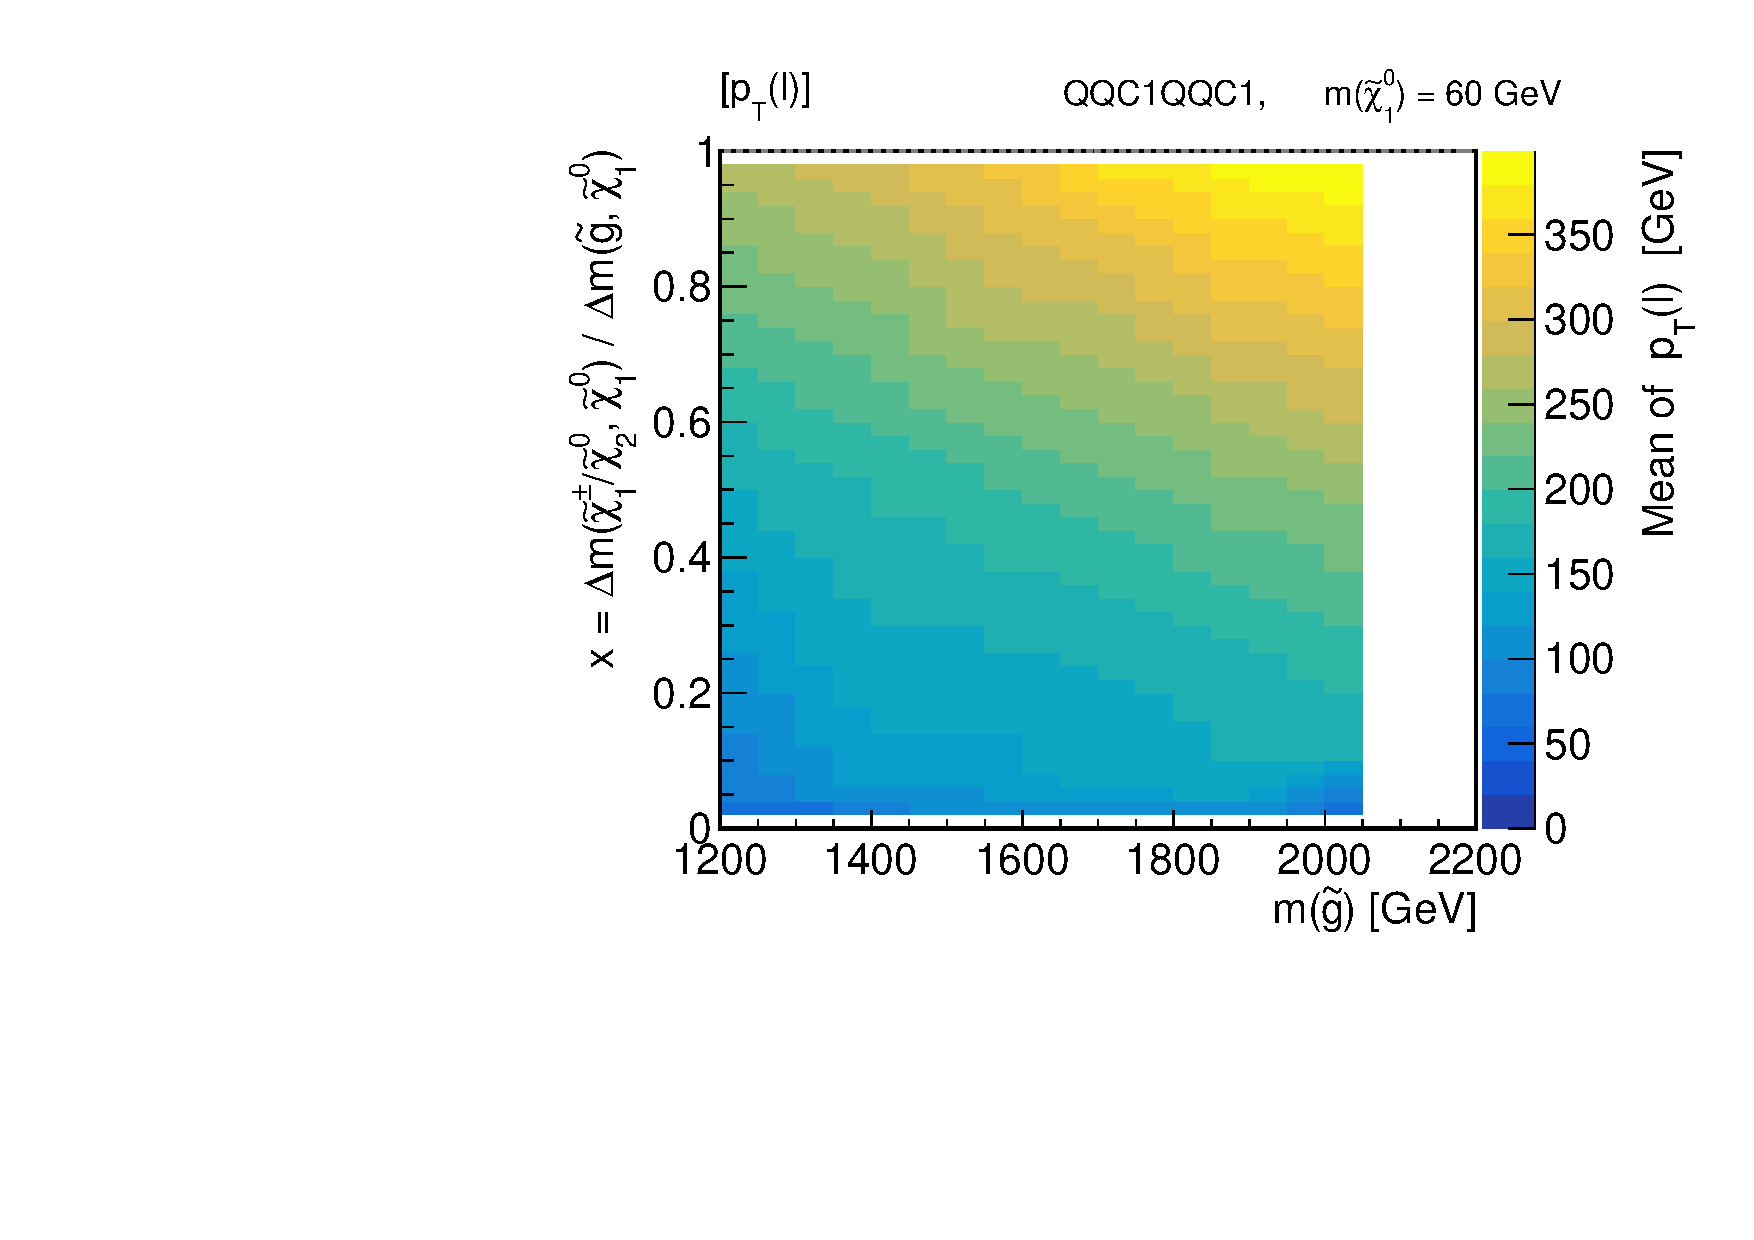
\includegraphics[width=0.45\textwidth]{figures/SRdefinition/kineMap/GG_symQQC1_varx_lep1Pt.pdf}}
    \subfigure[]{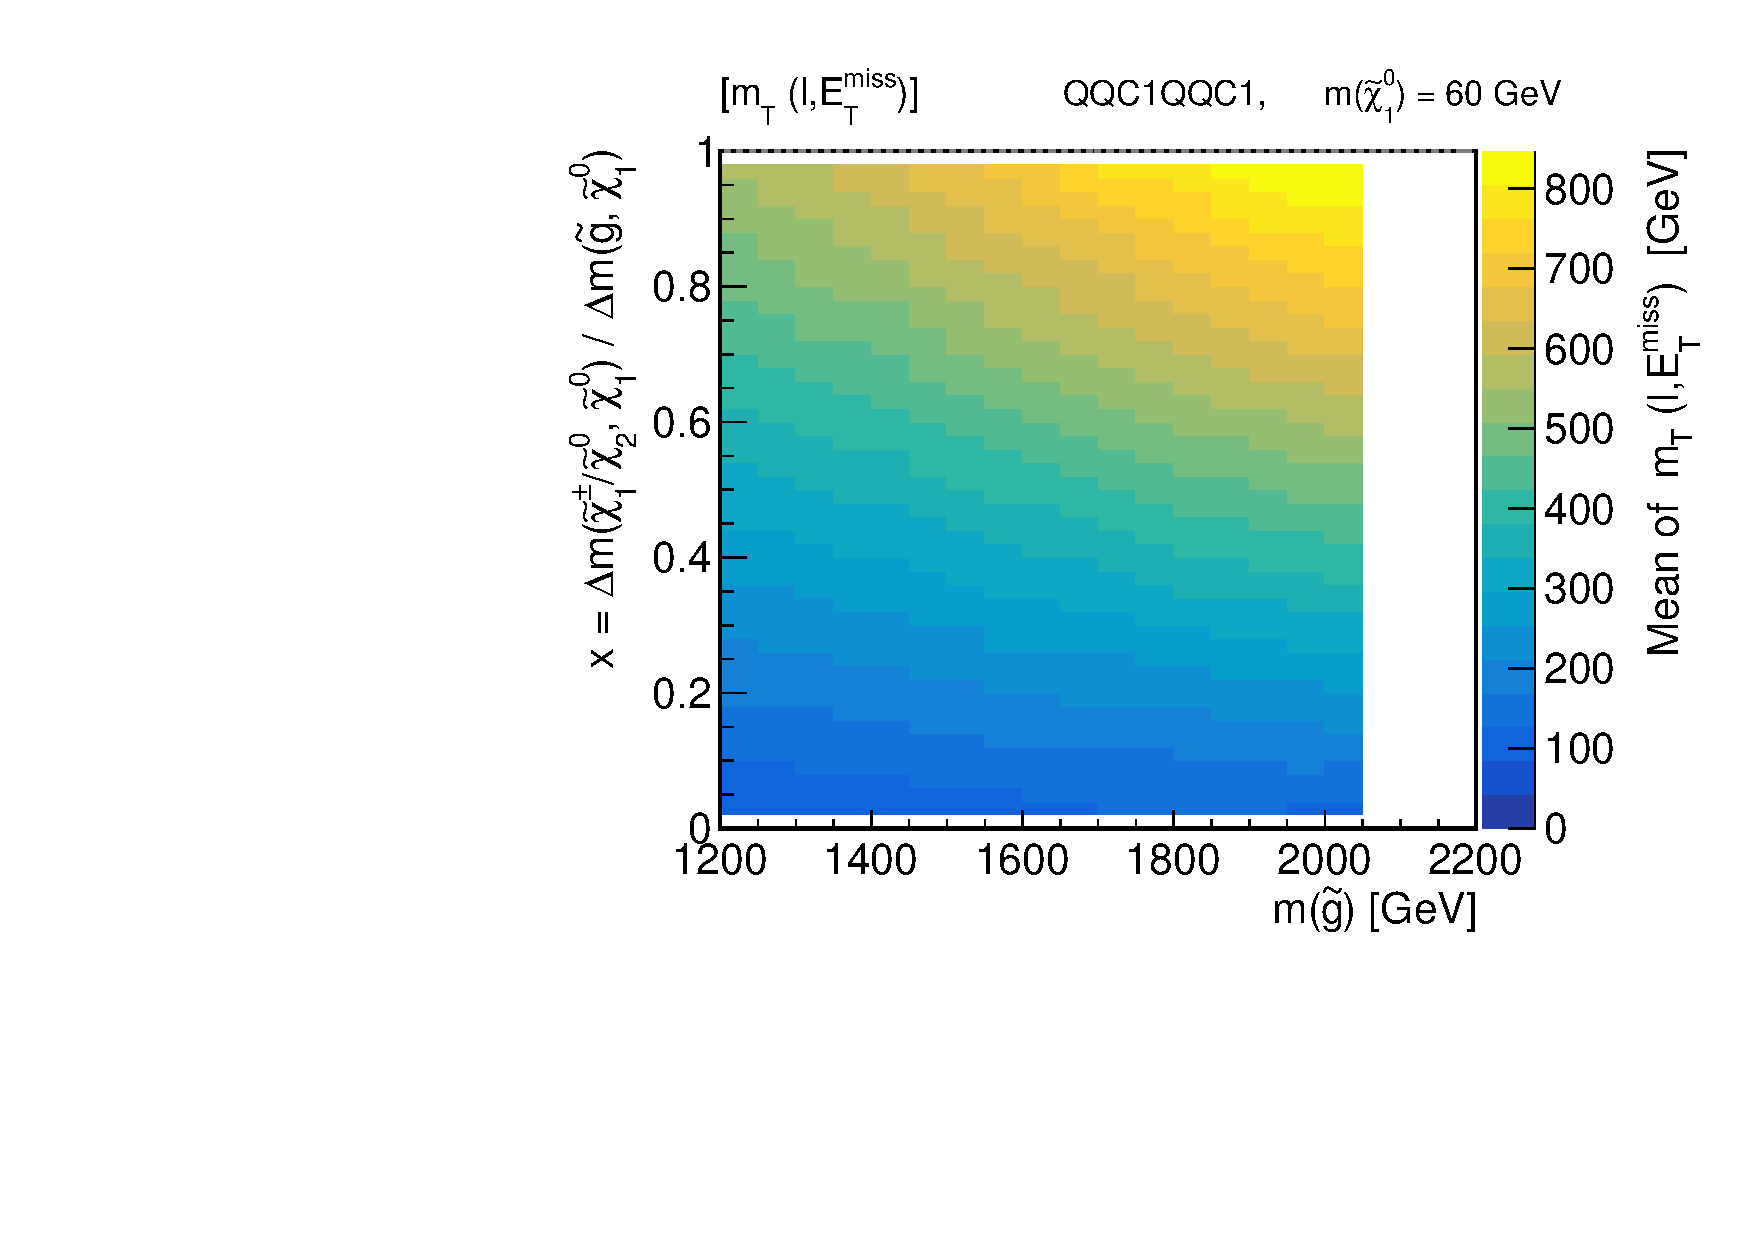
\includegraphics[width=0.45\textwidth]{figures/SRdefinition/kineMap/GG_symQQC1_varx_mt.pdf}}
    \subfigure[]{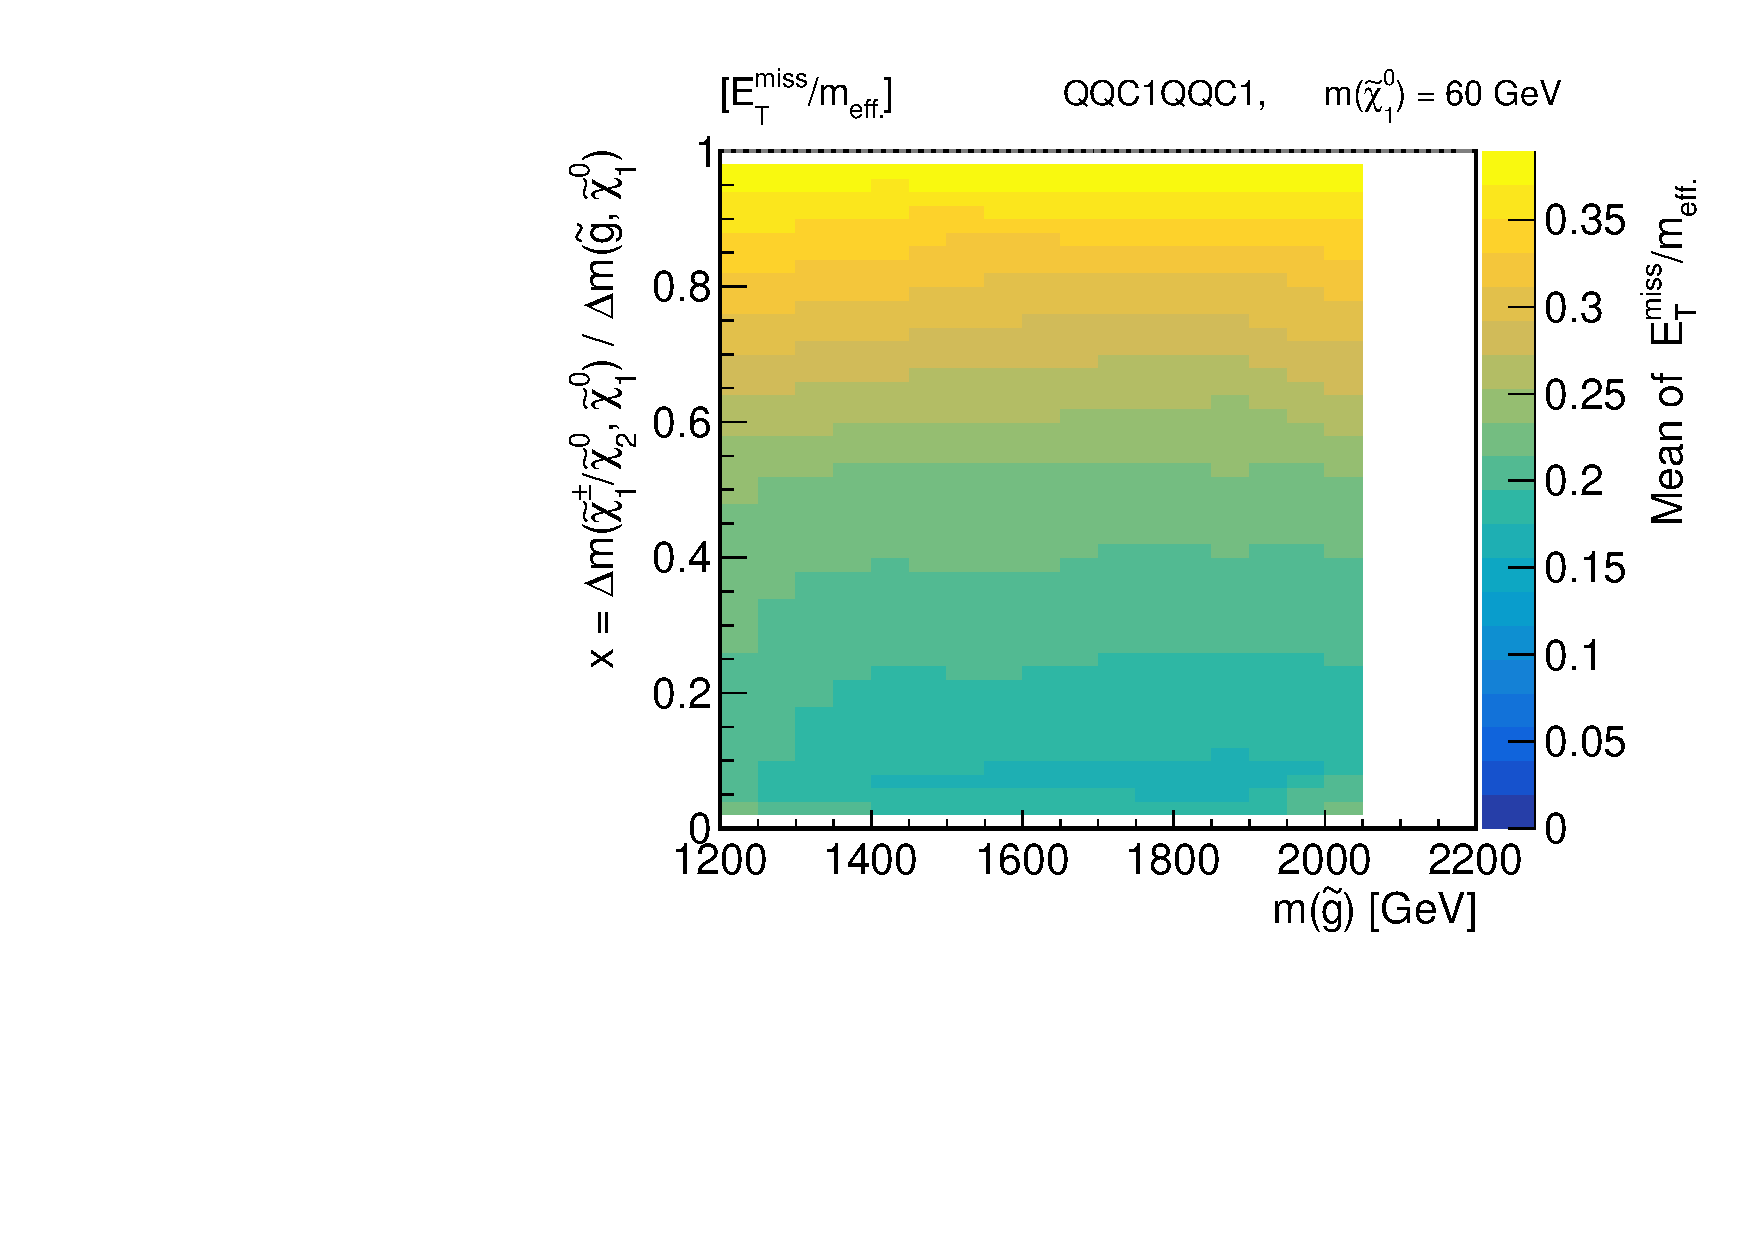
\includegraphics[width=0.45\textwidth]{figures/SRdefinition/kineMap/GG_symQQC1_varx_metOverMeff.pdf}}
    \subfigure[]{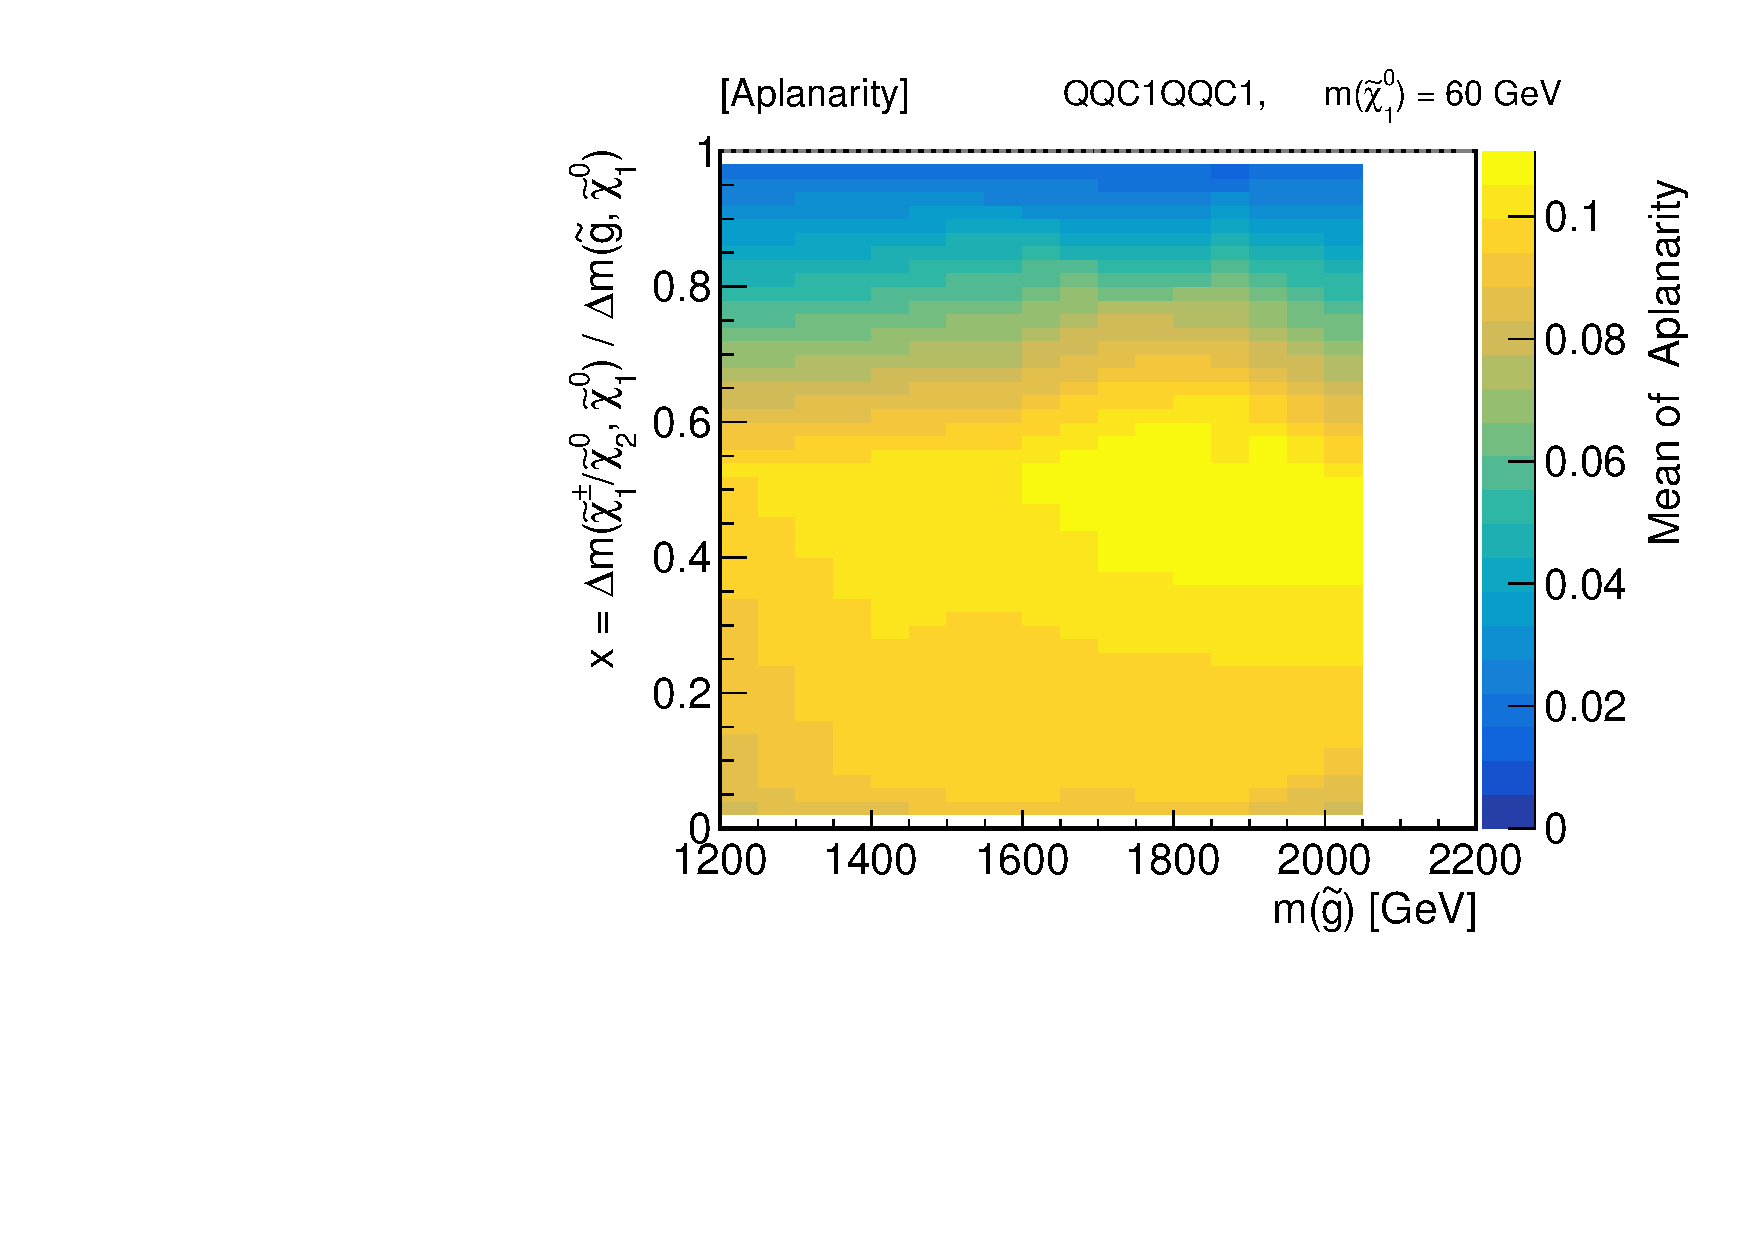
\includegraphics[width=0.45\textwidth]{figures/SRdefinition/kineMap/GG_symQQC1_varx_LepAplanarity.pdf}}
    \caption{ Mean of (a) $\meffInc$ (b) $\met$ (c) $\lepPt$ (d) $\mt$ (e) $\metOverMeff$  (f) aplanarity, for the QQC1QQC1 \varx grid, after the pre-selection. 
      \label{fig::SRdefinition::kineMap_QQC1QQC1_varx} 
    }
\end{figure}

 
%\begin{figure}[h]
%  \centering
%    \subfigure[]{\includegraphics[width=0.45\textwidth]{figures/SRdefinition/kineMap/GG_symQQC1_dM20_nJet30.pdf}}
%    \subfigure[]{\includegraphics[width=0.45\textwidth]{figures/SRdefinition/kineMap/GG_symQQC1_dM20_meff.pdf}}
%    \subfigure[]{\includegraphics[width=0.45\textwidth]{figures/SRdefinition/kineMap/GG_symQQC1_dM20_met.pdf}}
%    \subfigure[]{\includegraphics[width=0.45\textwidth]{figures/SRdefinition/kineMap/GG_symQQC1_dM20_lep1Pt.pdf}}
%    \subfigure[]{\includegraphics[width=0.45\textwidth]{figures/SRdefinition/kineMap/GG_symQQC1_dM20_mt.pdf}}
%    \subfigure[]{\includegraphics[width=0.45\textwidth]{figures/SRdefinition/kineMap/GG_symQQC1_dM20_LepAplanarity.pdf}}
%    \caption{ Mean of (a) jet-multiplicity ($p_T>30\gev$) (b) $\meffInc$ (c) $\met$ (d) $\lepPt$ (e) $\mt$ (f) aplanarity, for the QQC1QQC1 $\Delta M = 20\gev$ grid, after the pre-selection. }
%\end{figure}
 
\begin{figure}[h]
  \centering
%    \subfigure[]{\includegraphics[width=0.45\textwidth]{figures/SRdefinition/kineMap/GG_symQQC1_dM30_nJet30.pdf}}
    \subfigure[]{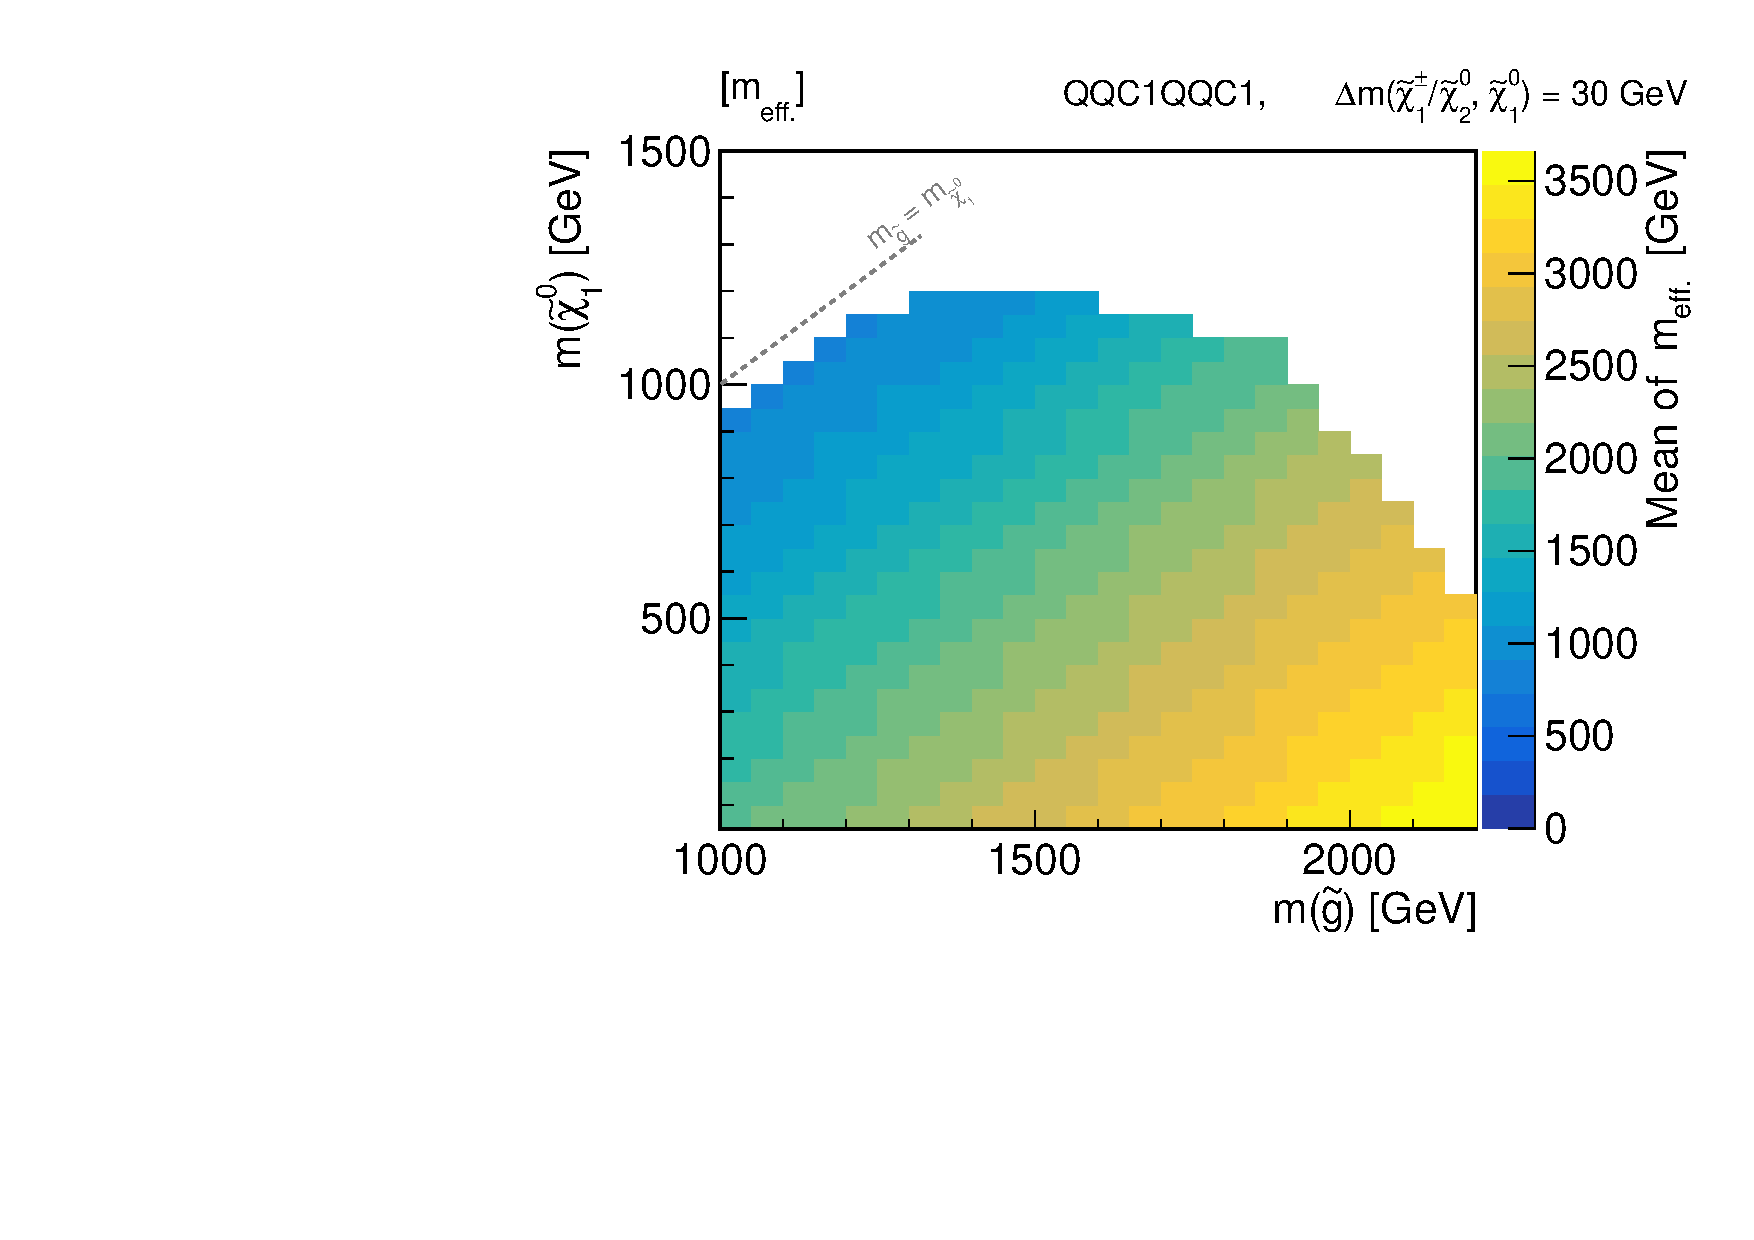
\includegraphics[width=0.45\textwidth]{figures/SRdefinition/kineMap/GG_symQQC1_dM30_meff.pdf}}
    \subfigure[]{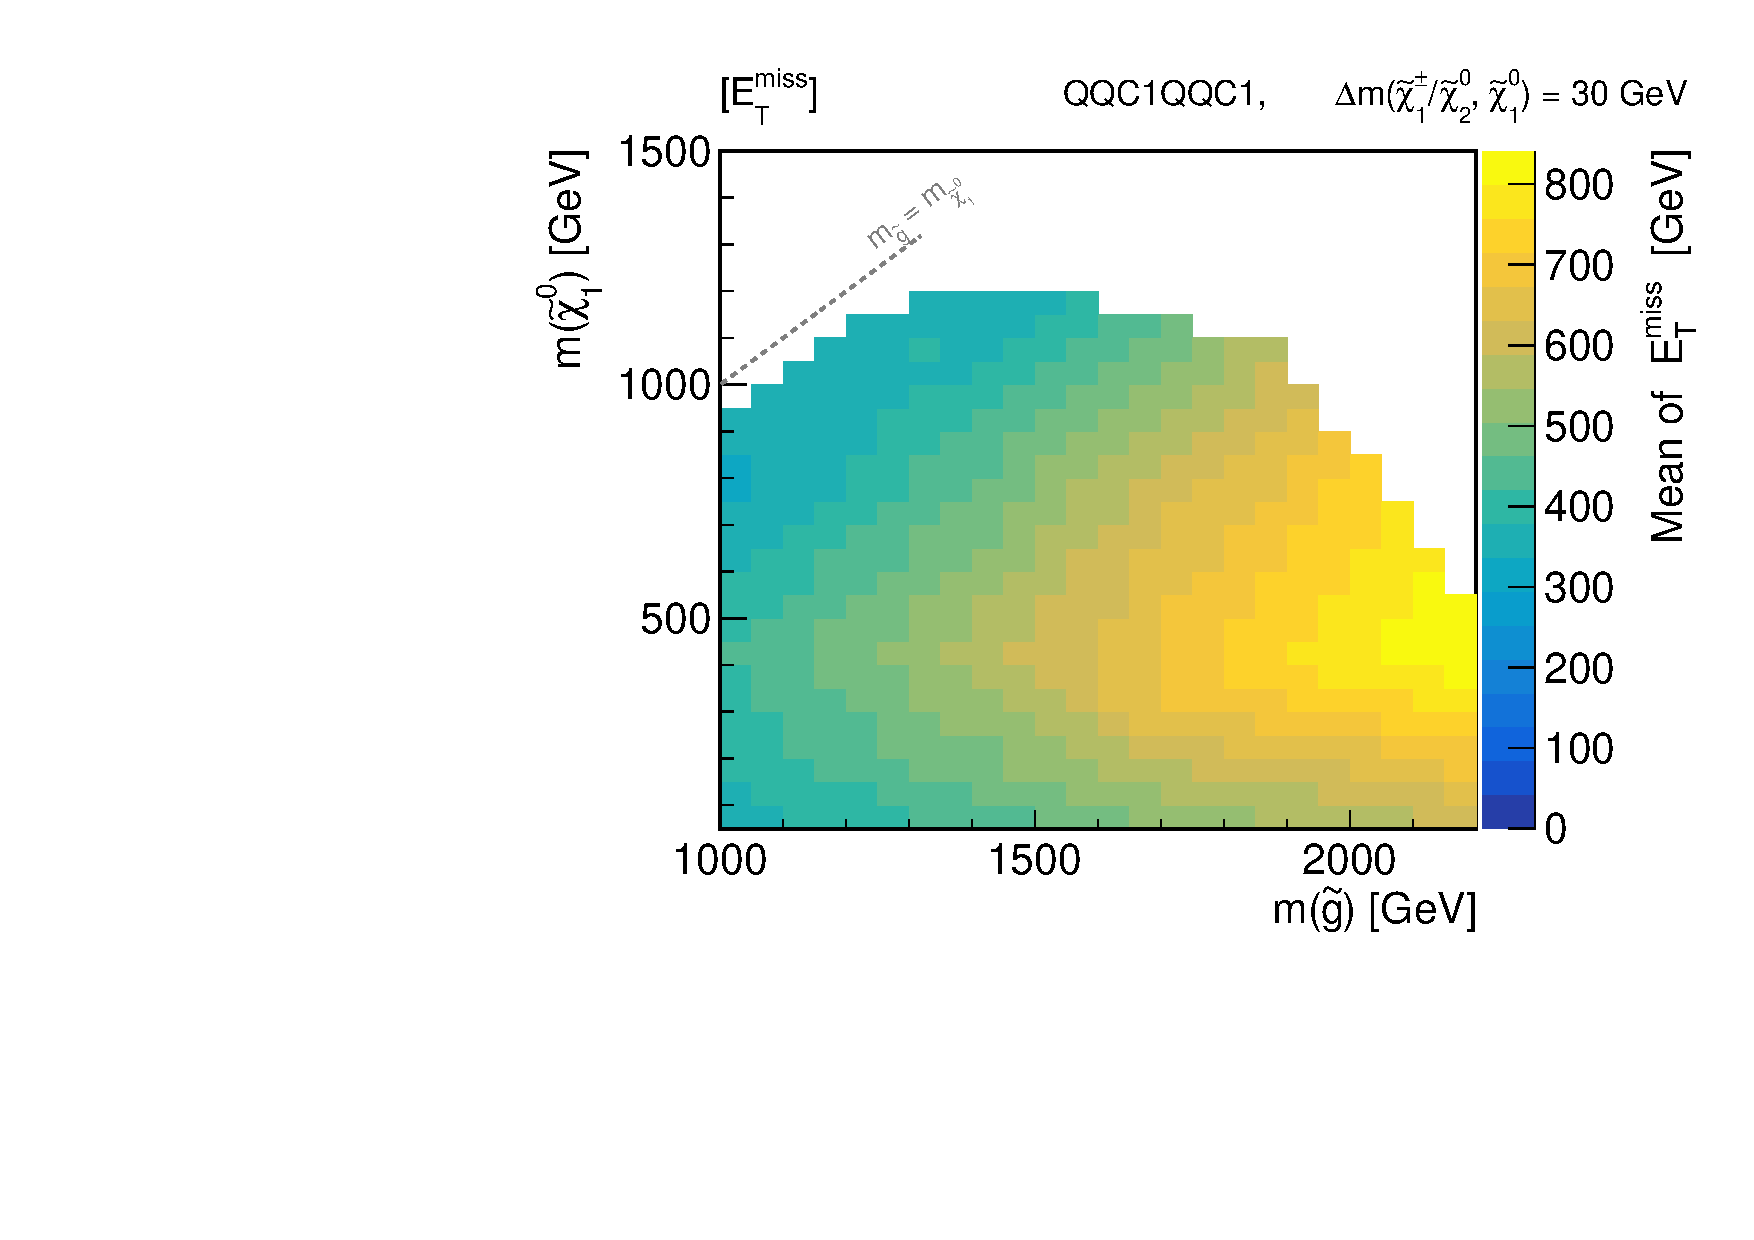
\includegraphics[width=0.45\textwidth]{figures/SRdefinition/kineMap/GG_symQQC1_dM30_met.pdf}}
    \subfigure[]{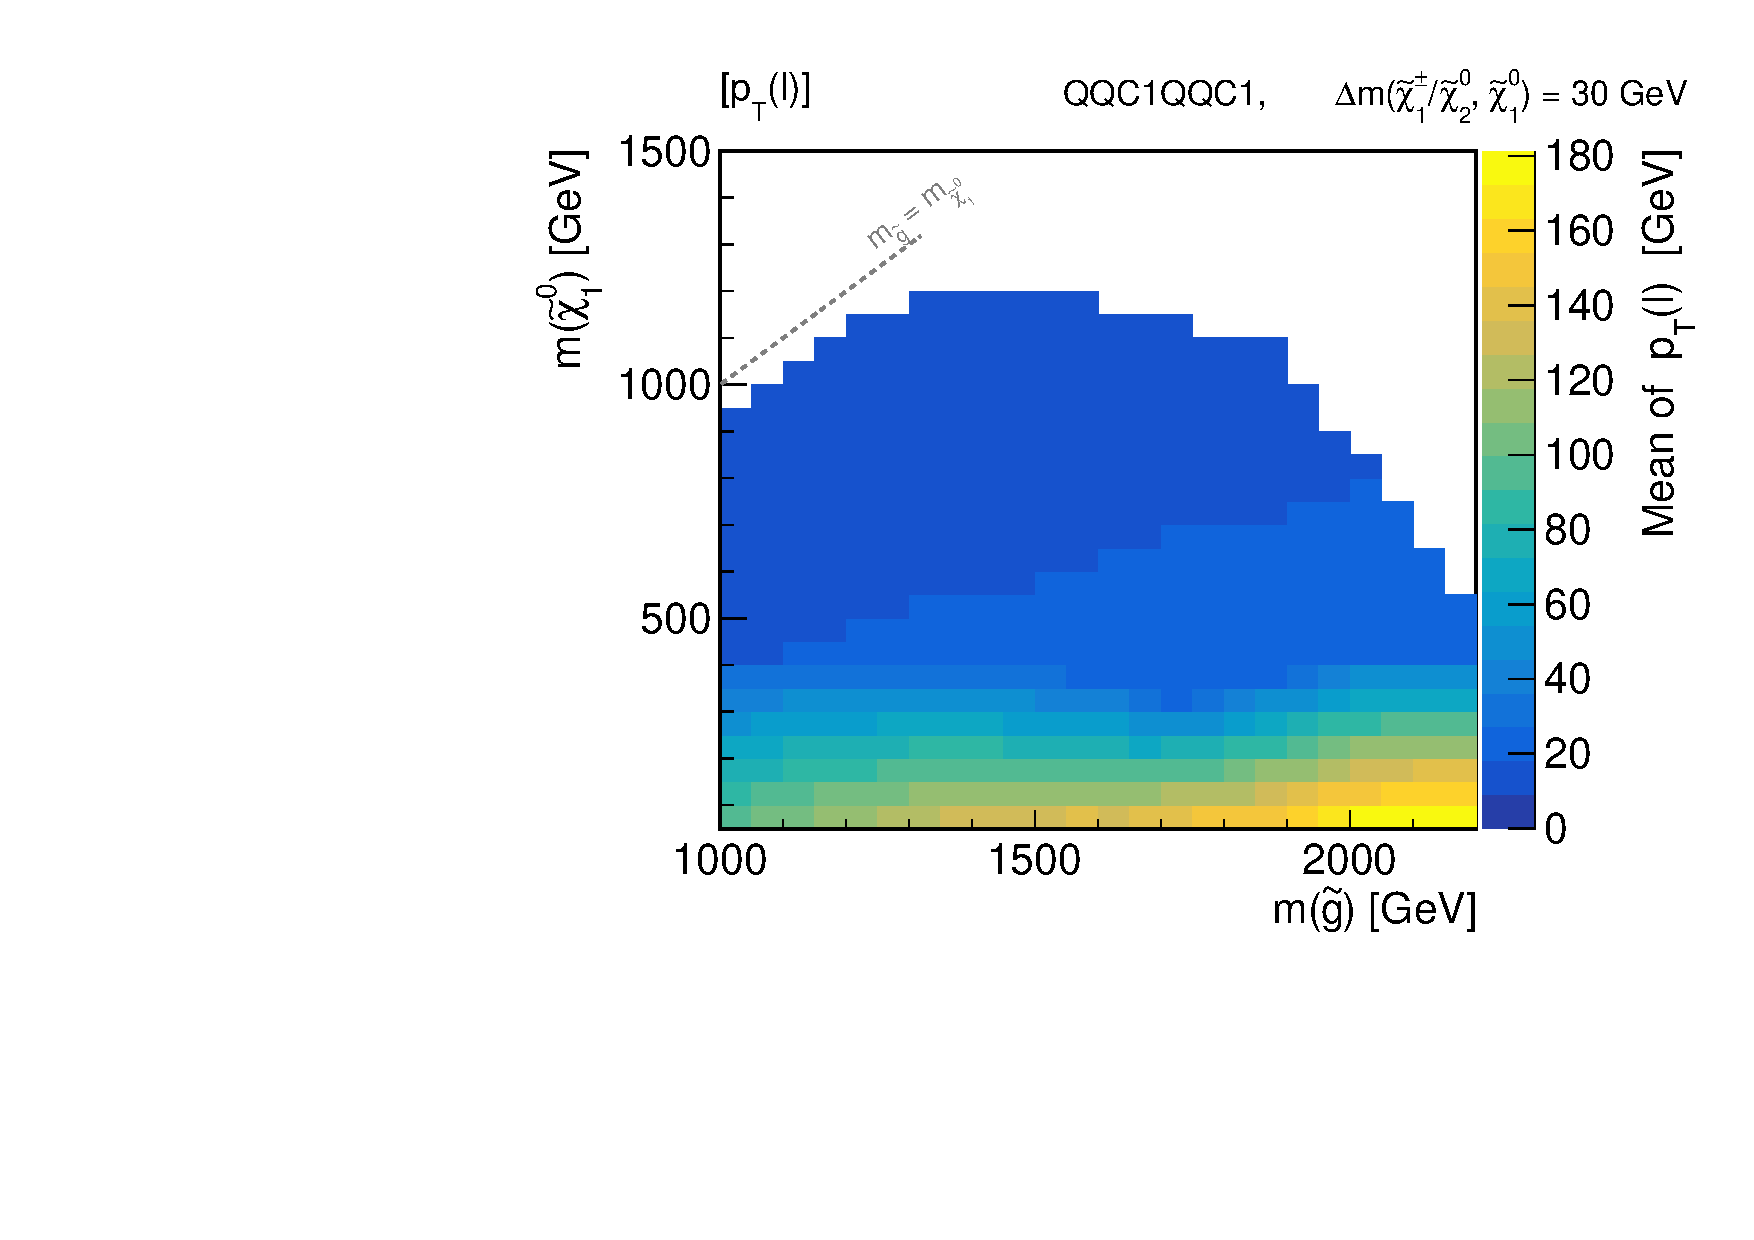
\includegraphics[width=0.45\textwidth]{figures/SRdefinition/kineMap/GG_symQQC1_dM30_lep1Pt.pdf}}
    \subfigure[]{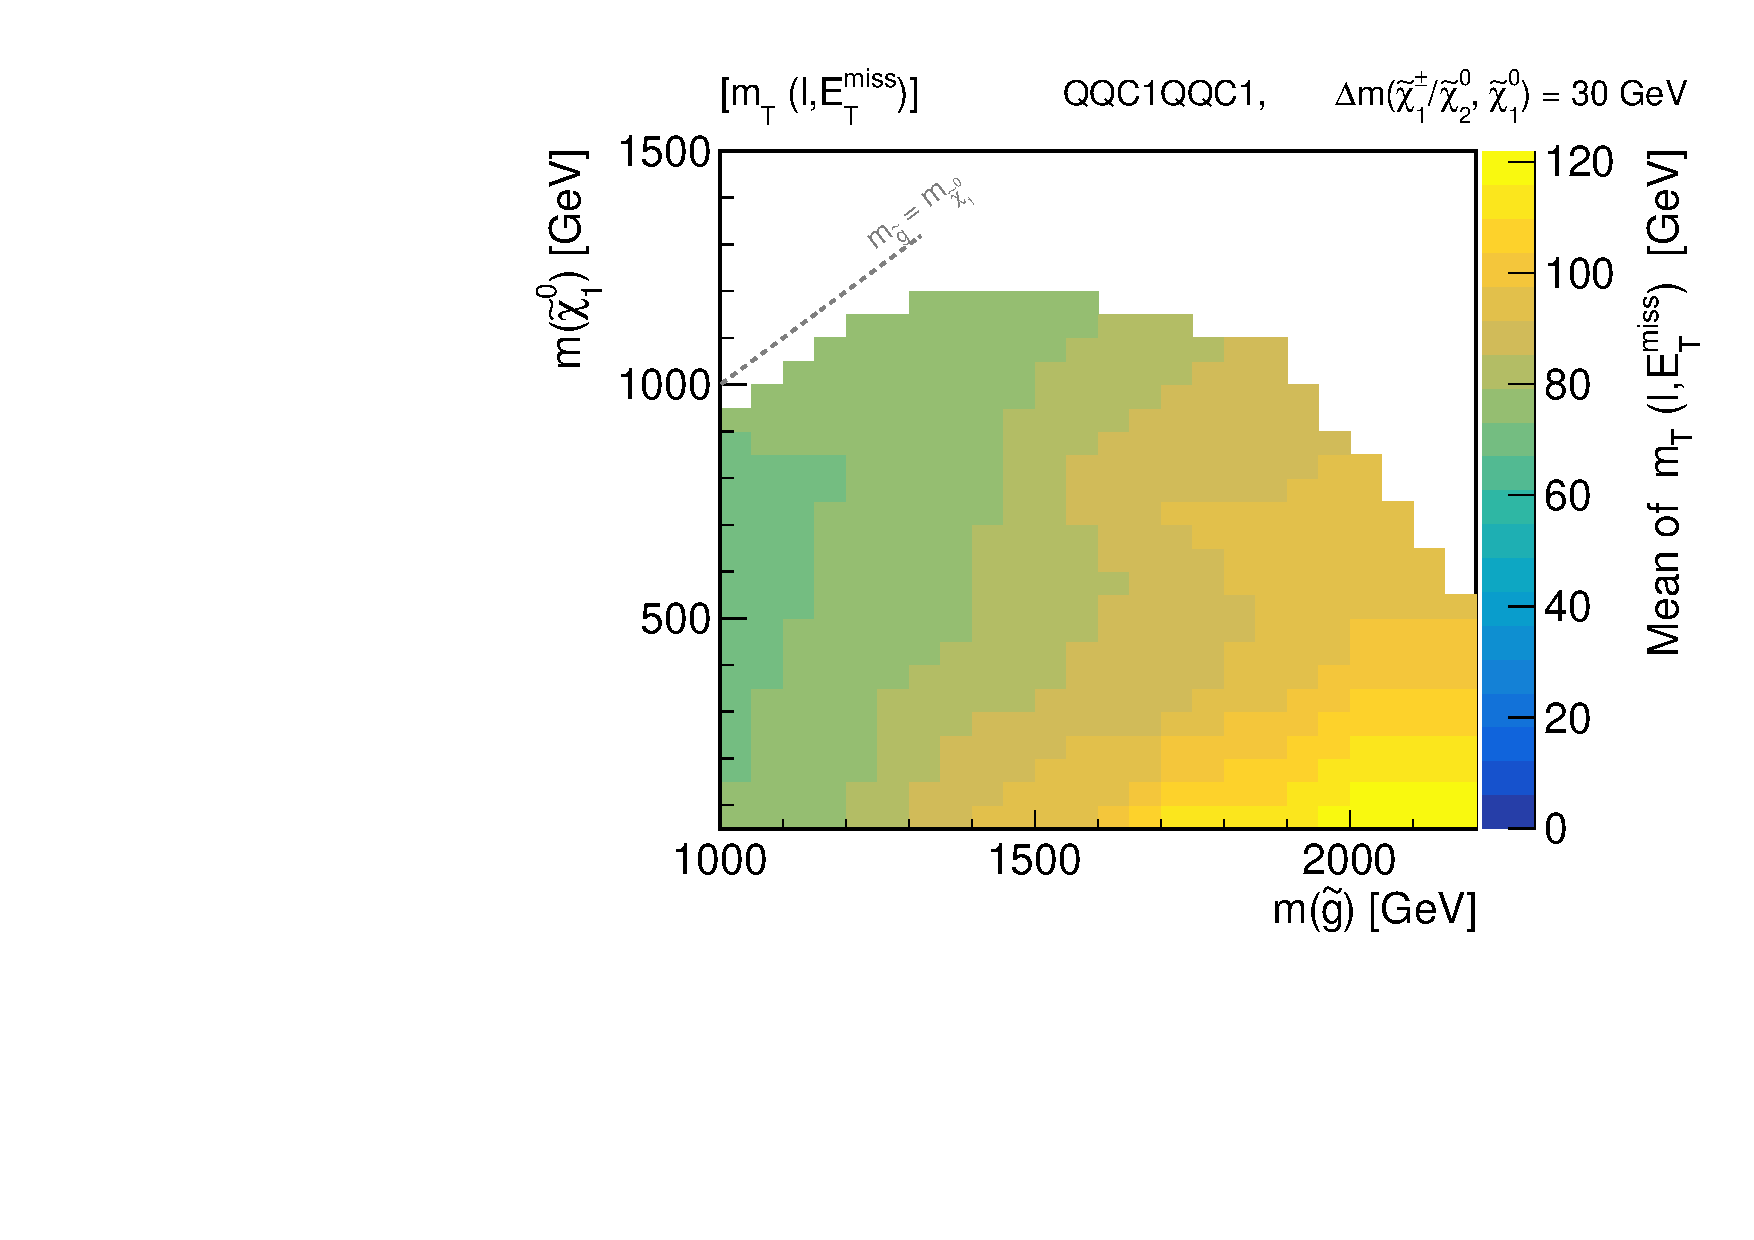
\includegraphics[width=0.45\textwidth]{figures/SRdefinition/kineMap/GG_symQQC1_dM30_mt.pdf}}
    \subfigure[]{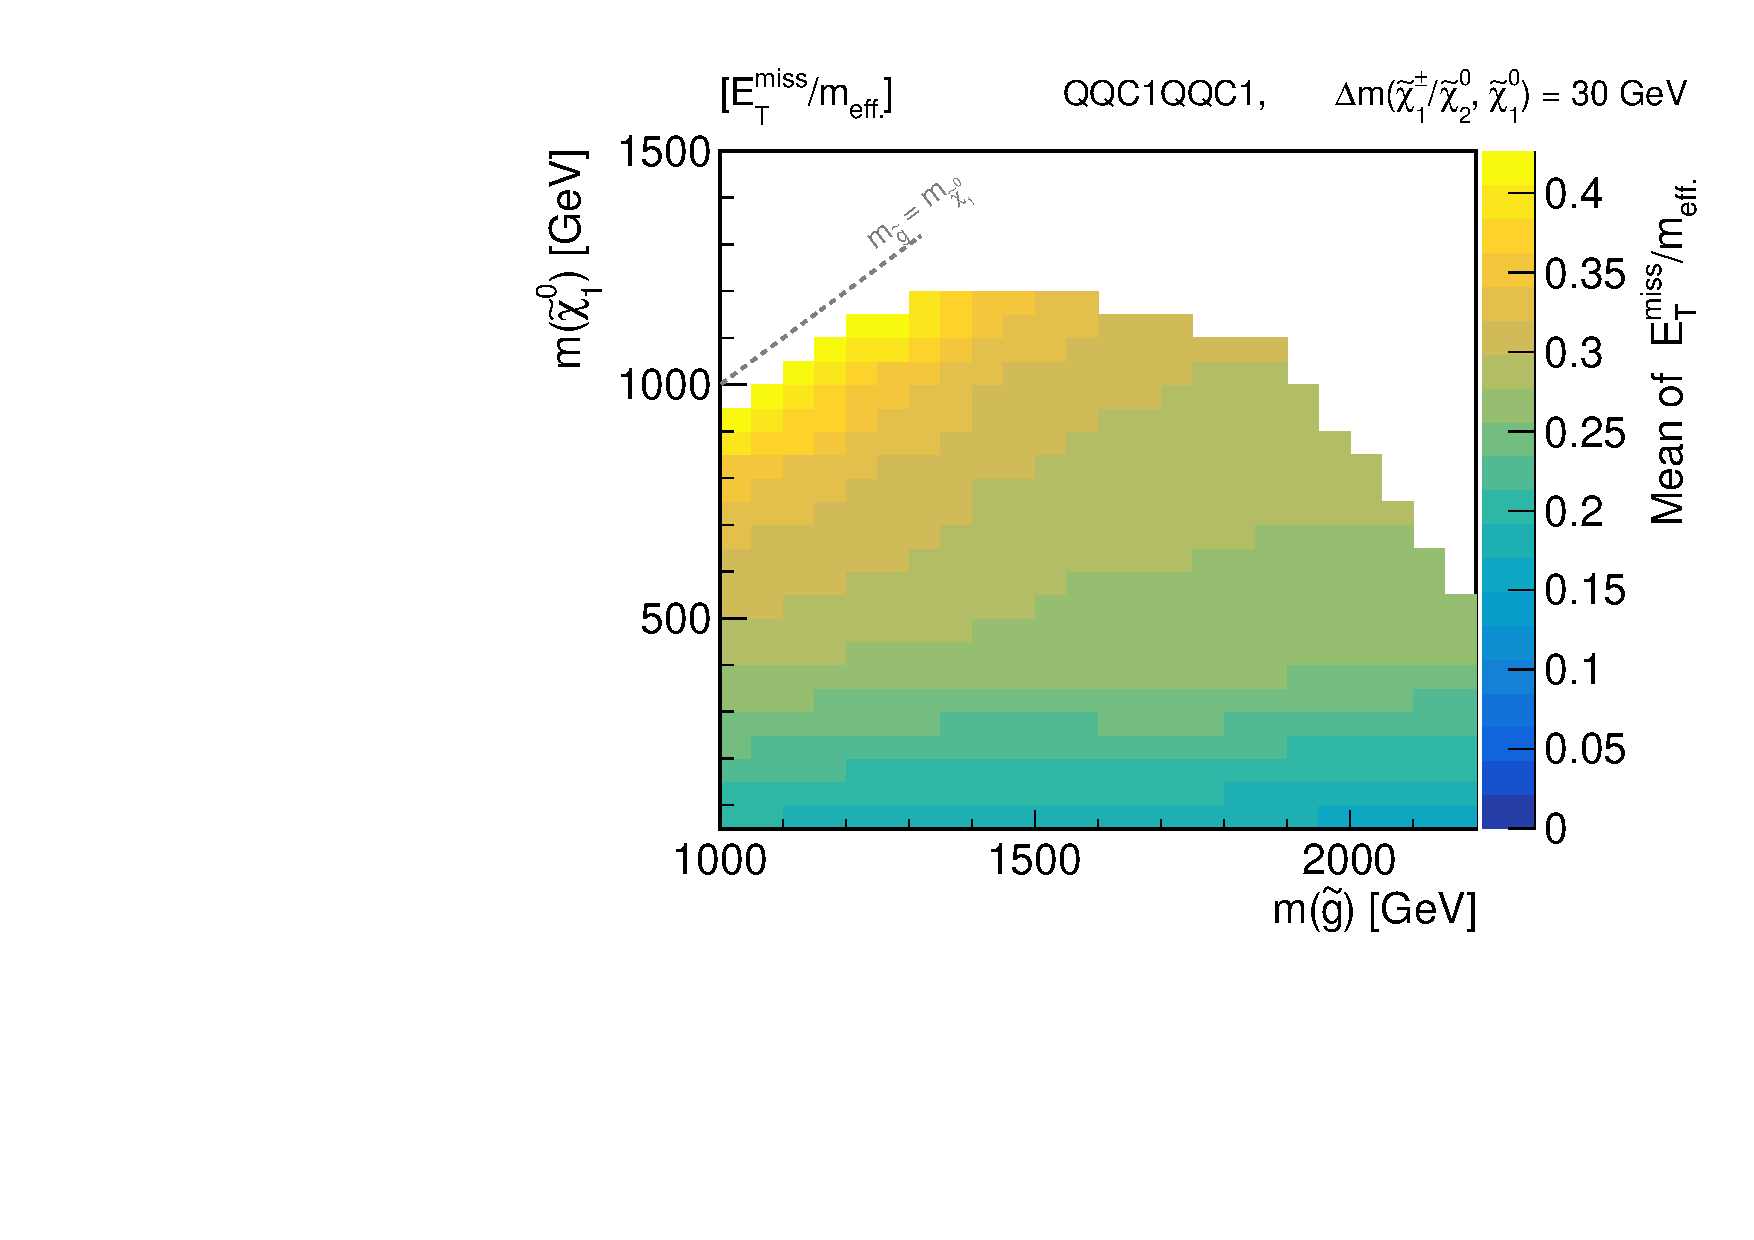
\includegraphics[width=0.45\textwidth]{figures/SRdefinition/kineMap/GG_symQQC1_dM30_metOverMeff.pdf}}
    \subfigure[]{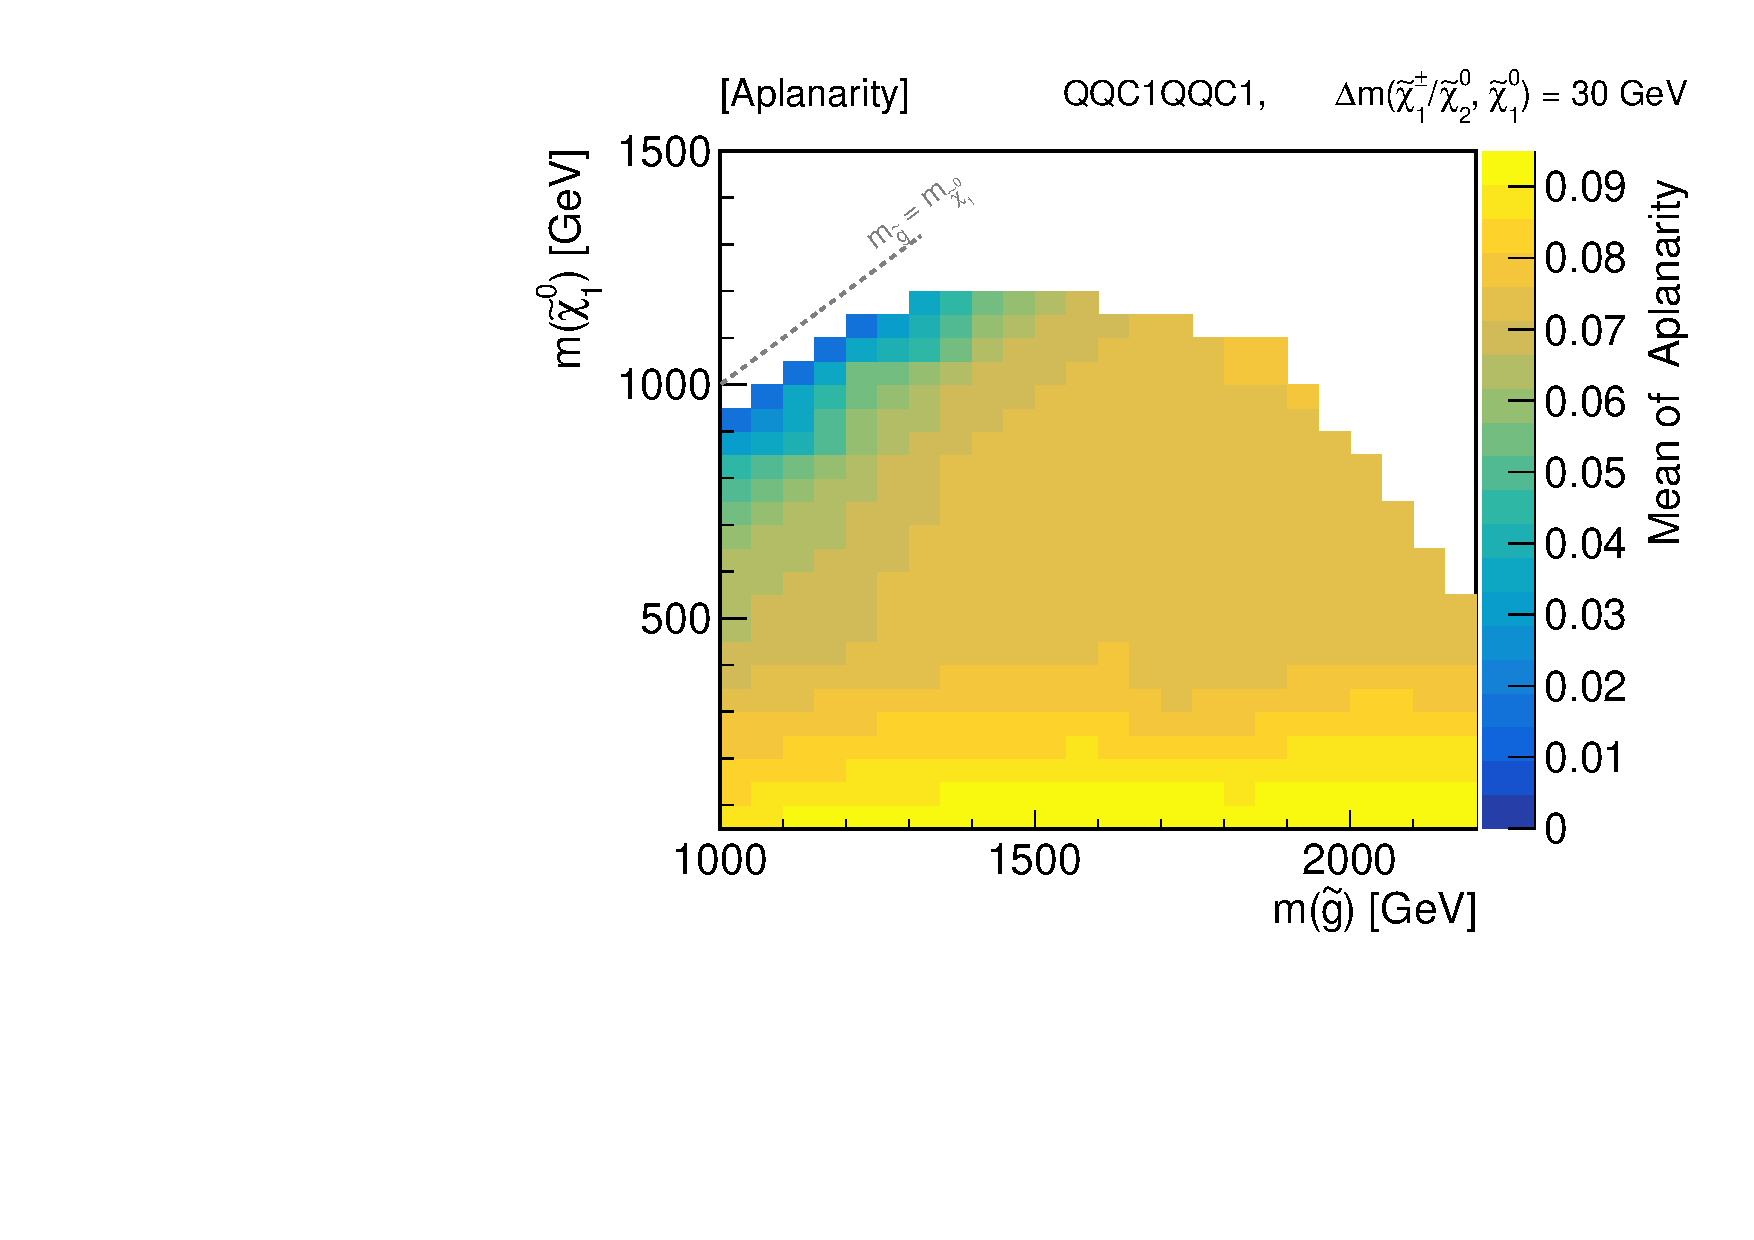
\includegraphics[width=0.45\textwidth]{figures/SRdefinition/kineMap/GG_symQQC1_dM30_LepAplanarity.pdf}}
    \caption{ Mean of (a) $\meffInc$ (b) $\met$ (c) $\lepPt$ (d) $\mt$ (e) $\metOverMeff$ (f) aplanarity, for the QQC1QQC1 \DMth grid, after the pre-selection. 
      \label{fig::SRdefinition::kineMap_QQC1QQC1_dM30} 
    }
\end{figure}


\begin{figure}[h]
  \centering
    \subfigure[]{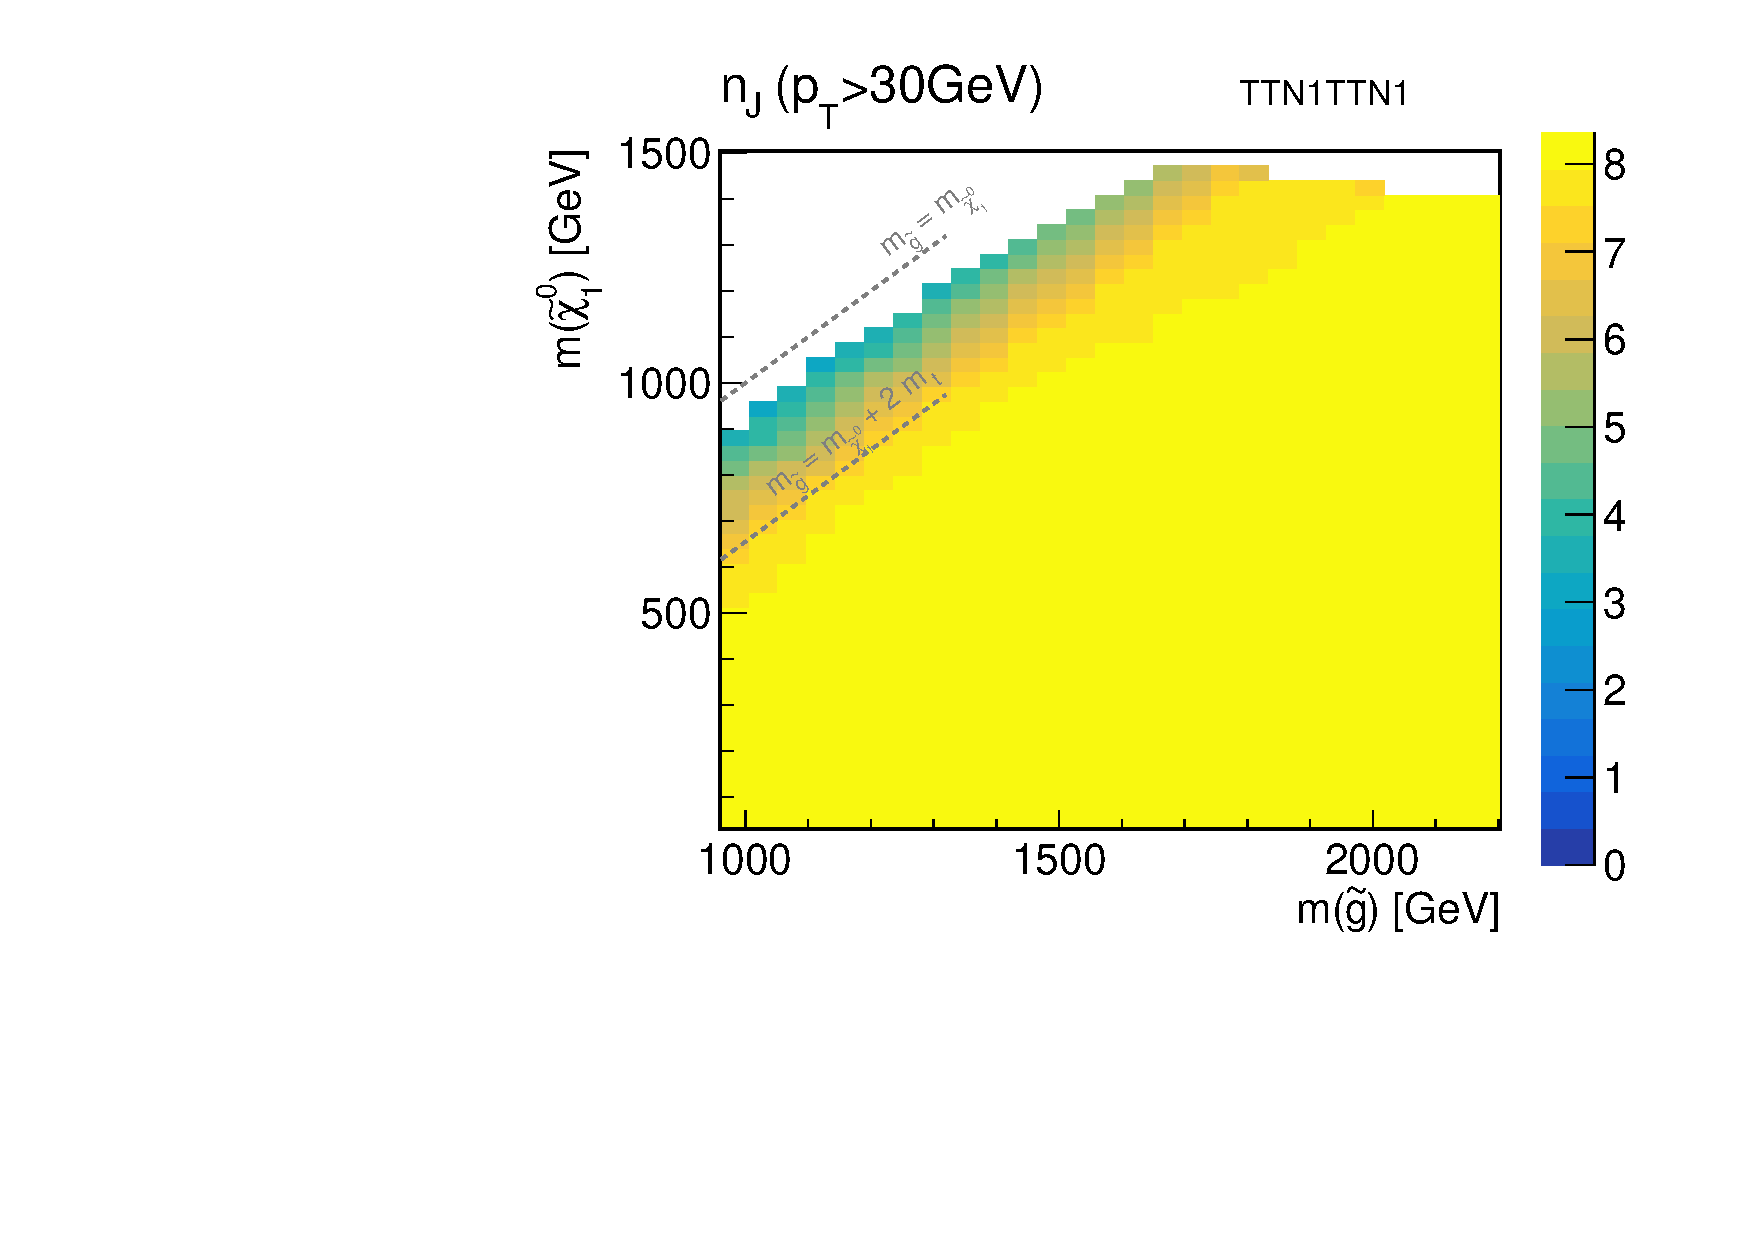
\includegraphics[width=0.32\textwidth]{figures/SRdefinition/kineMap/GG_symTTN1_x12_nJet30.pdf}}
    \subfigure[]{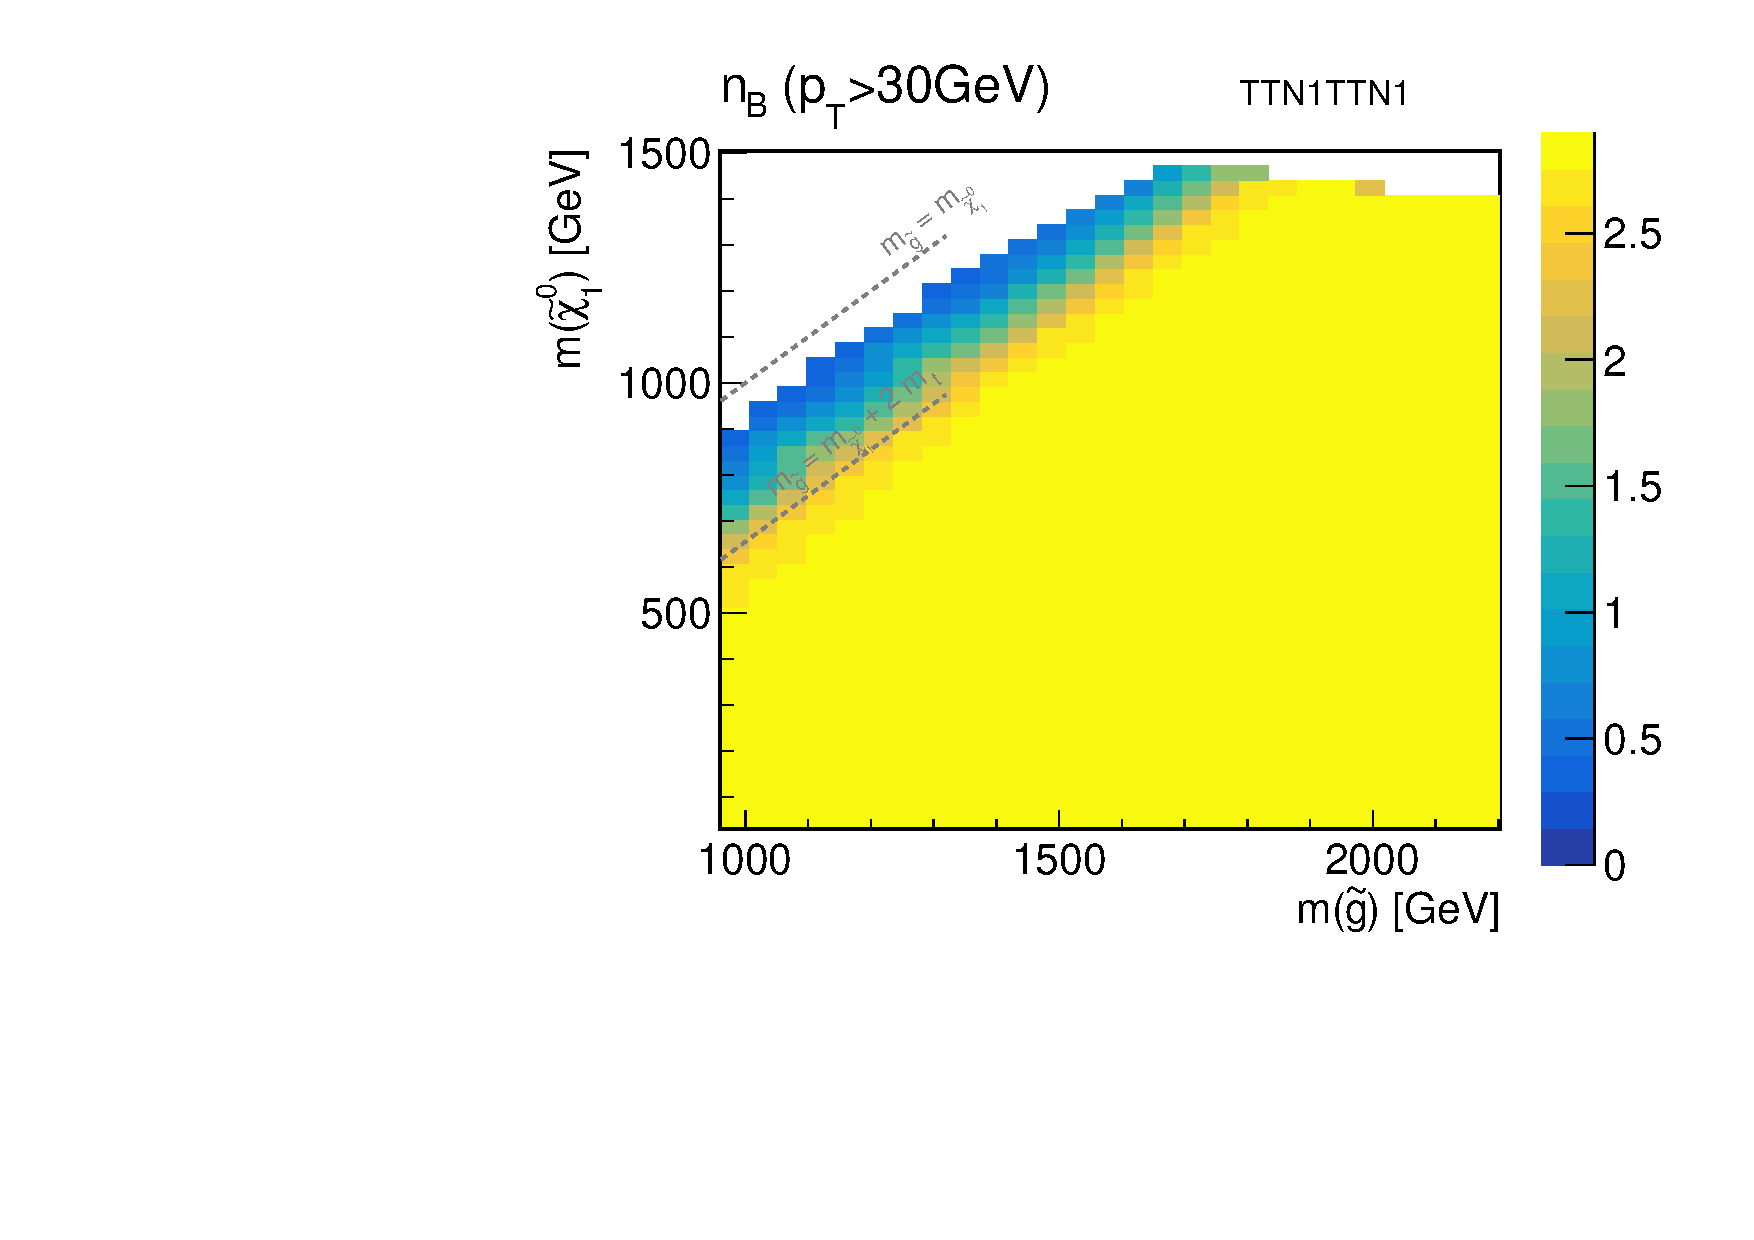
\includegraphics[width=0.32\textwidth]{figures/SRdefinition/kineMap/GG_symTTN1_x12_nBJet30.pdf}}
    \subfigure[]{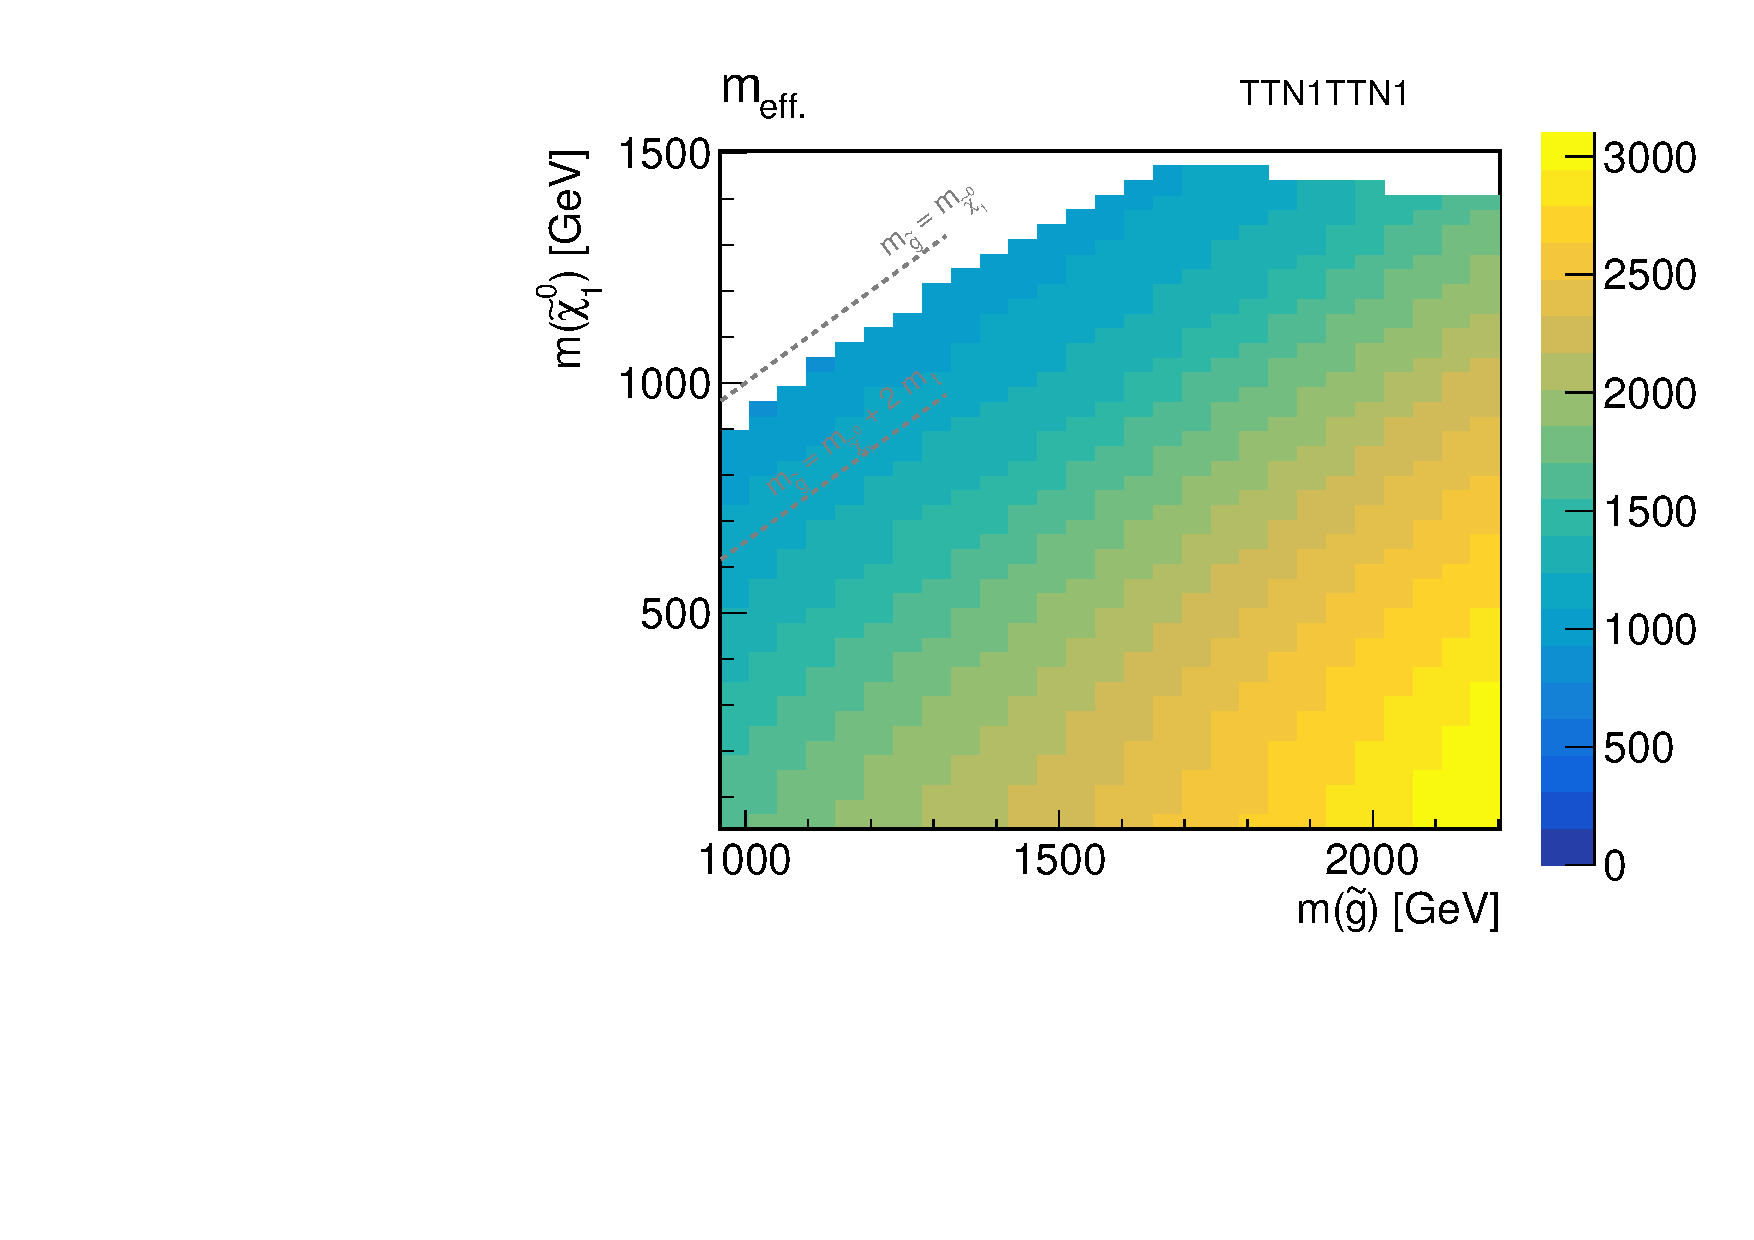
\includegraphics[width=0.32\textwidth]{figures/SRdefinition/kineMap/GG_symTTN1_x12_meff.pdf}}
    \subfigure[]{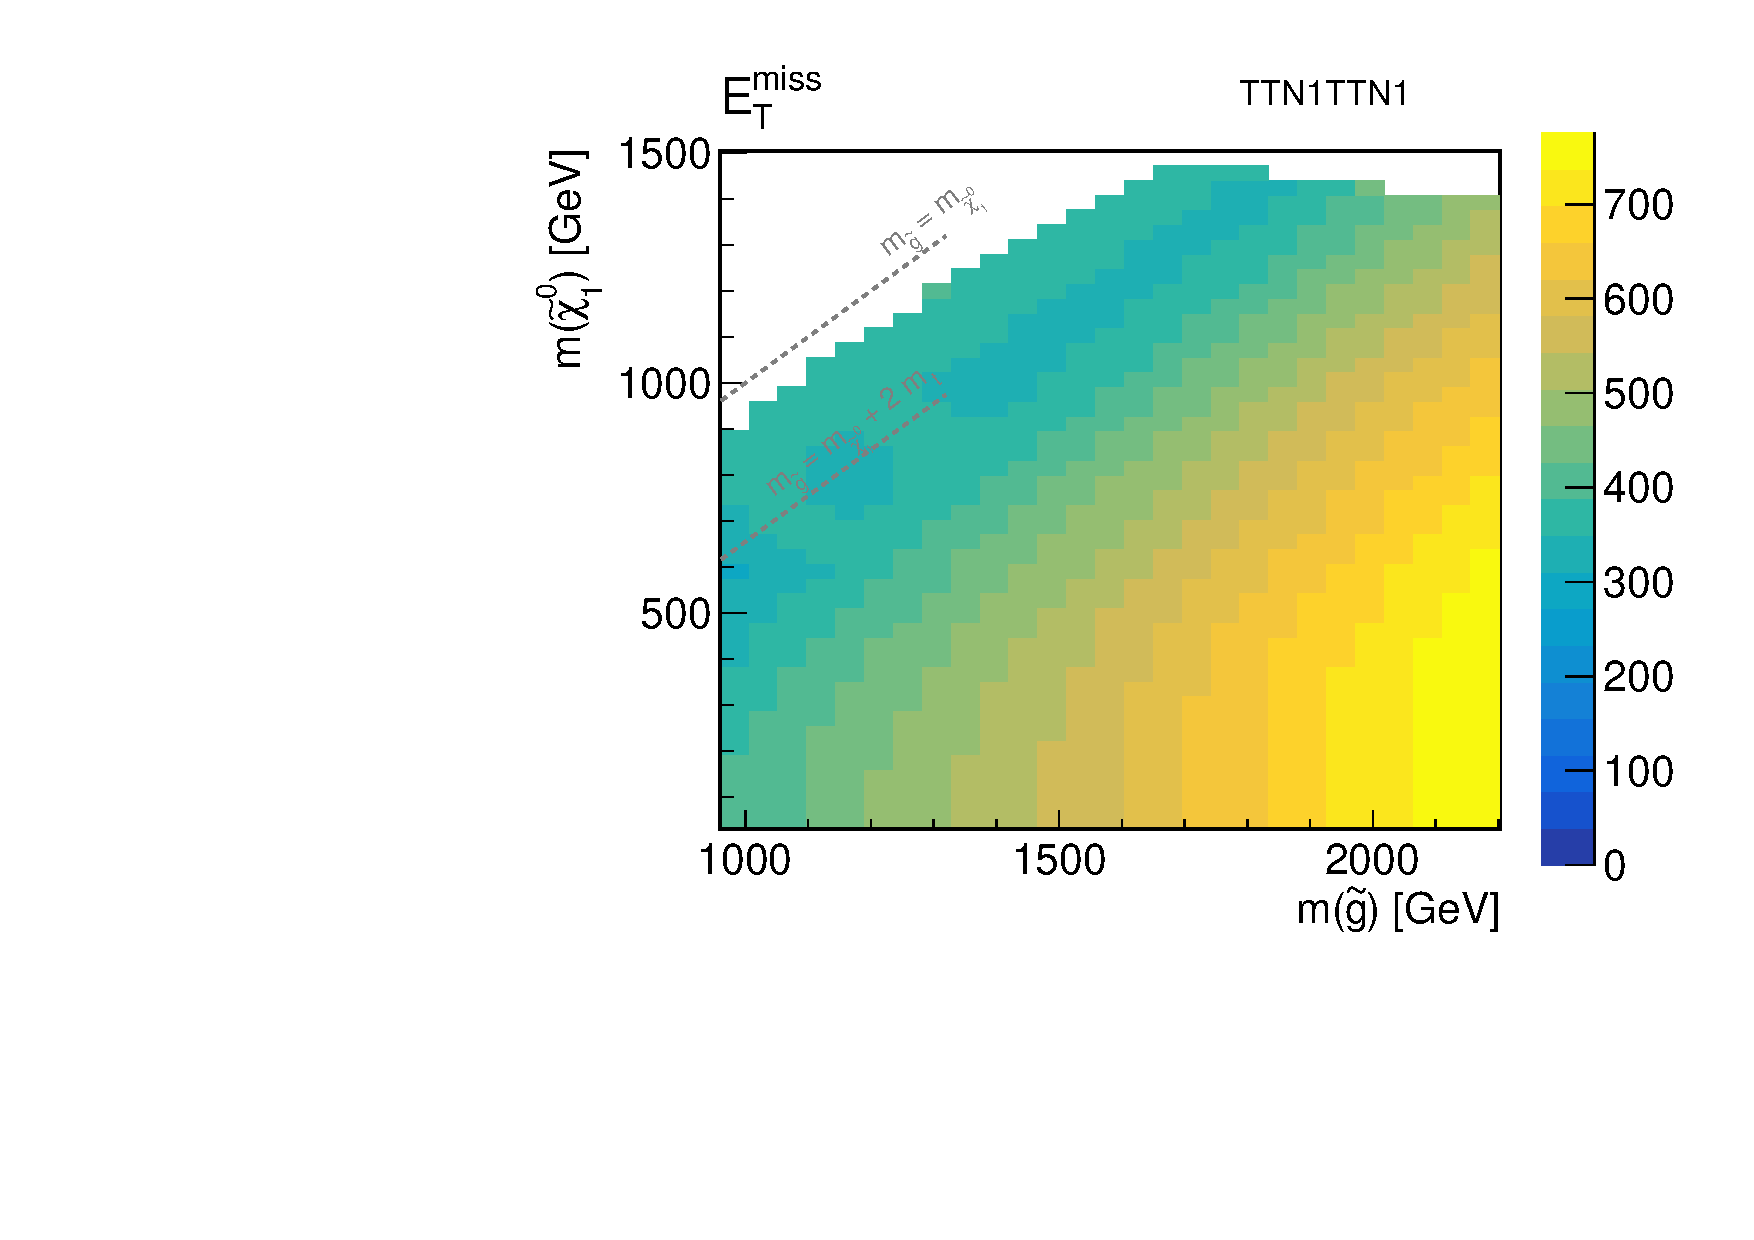
\includegraphics[width=0.32\textwidth]{figures/SRdefinition/kineMap/GG_symTTN1_x12_met.pdf}}
    \subfigure[]{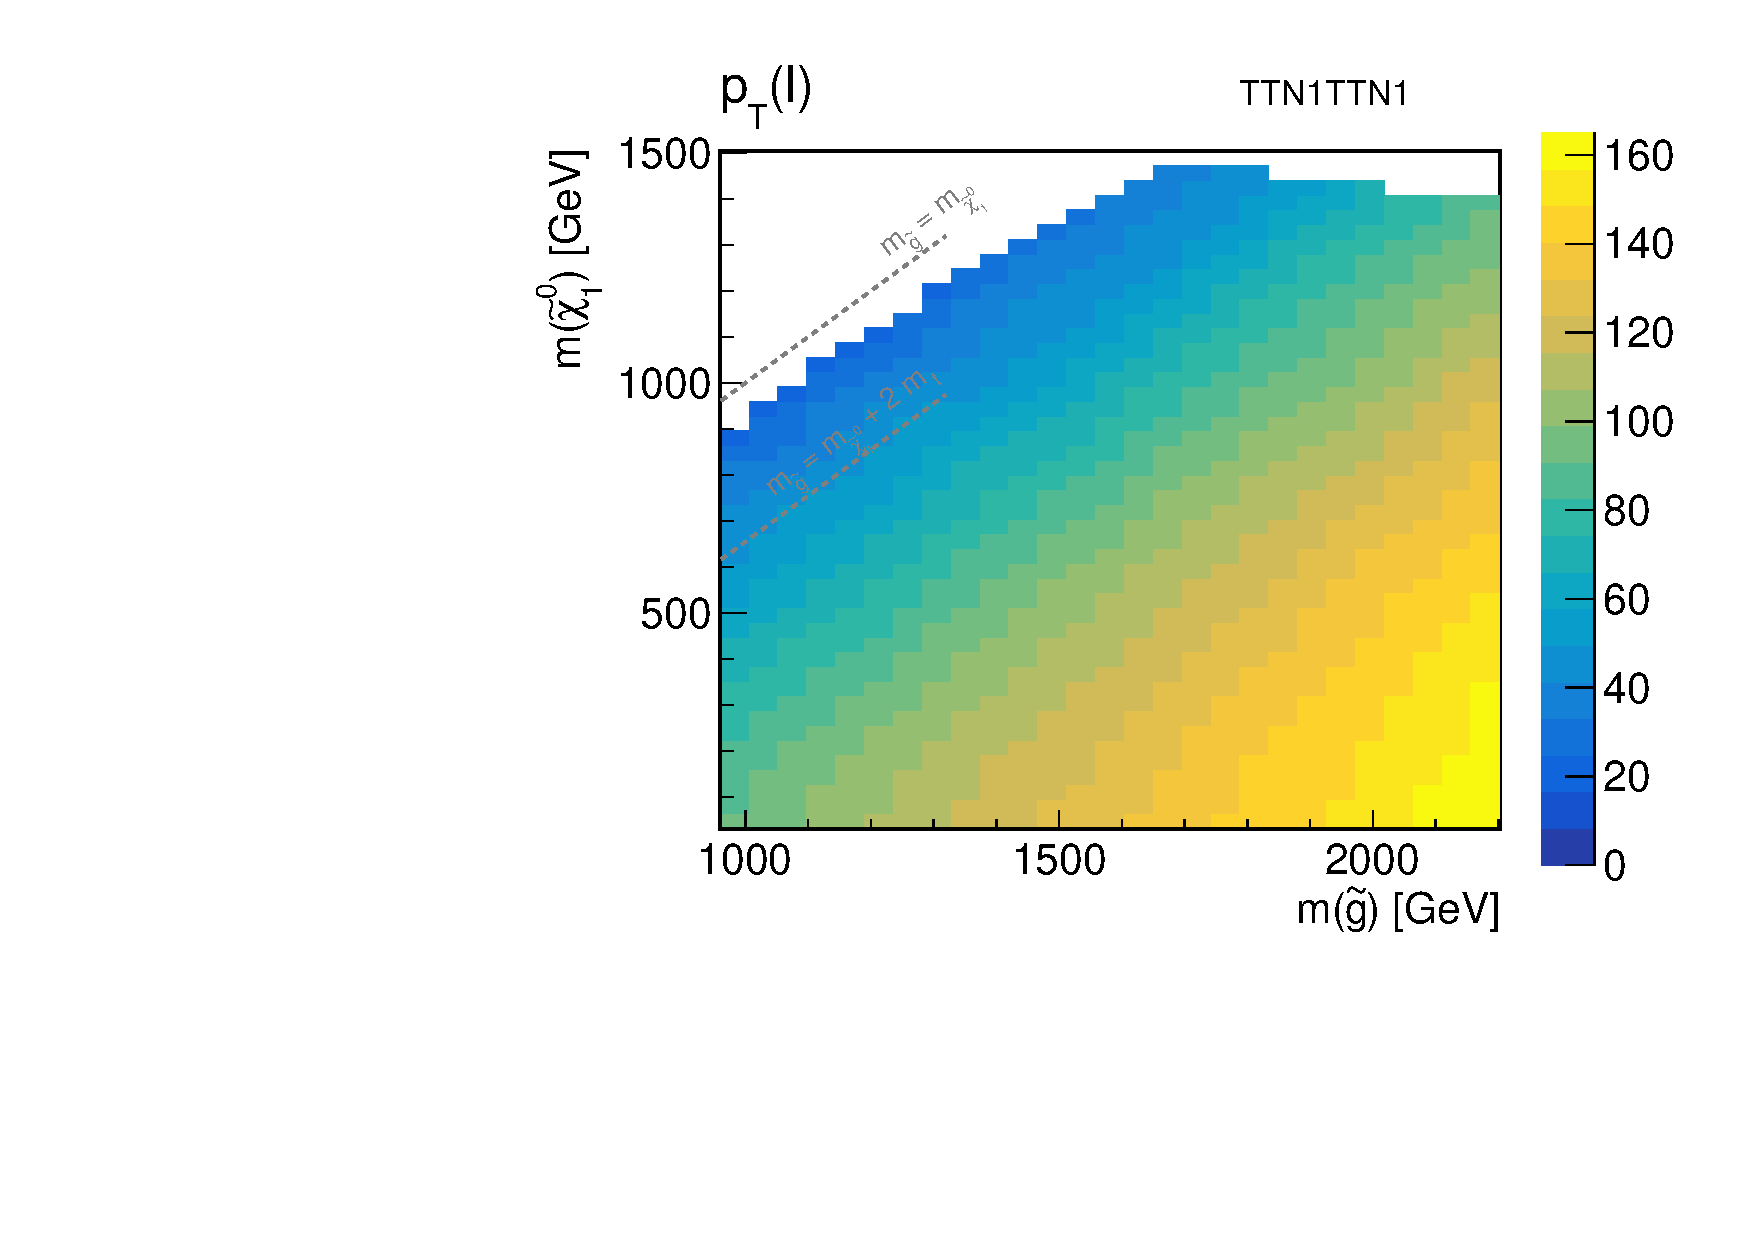
\includegraphics[width=0.32\textwidth]{figures/SRdefinition/kineMap/GG_symTTN1_x12_lep1Pt.pdf}}
    \subfigure[]{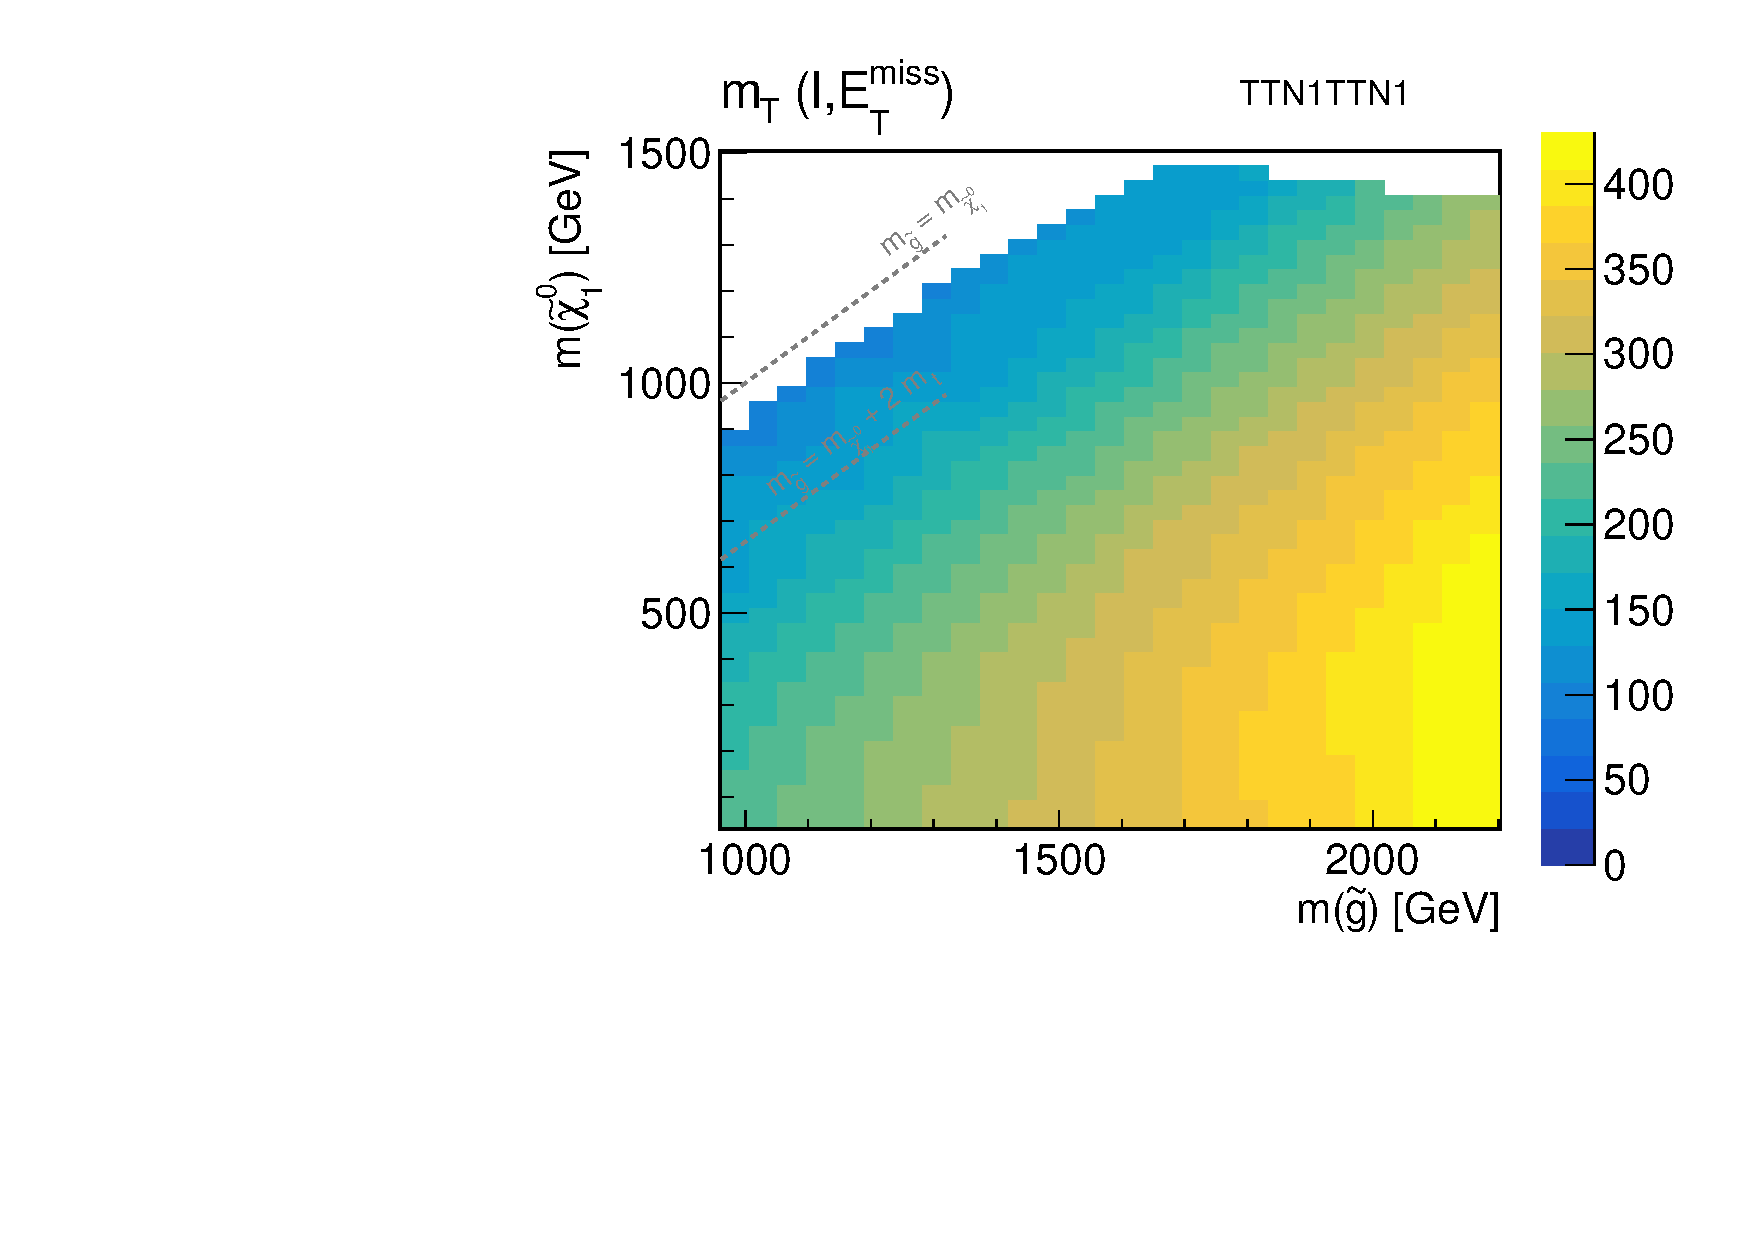
\includegraphics[width=0.32\textwidth]{figures/SRdefinition/kineMap/GG_symTTN1_x12_mt.pdf}}
    \subfigure[]{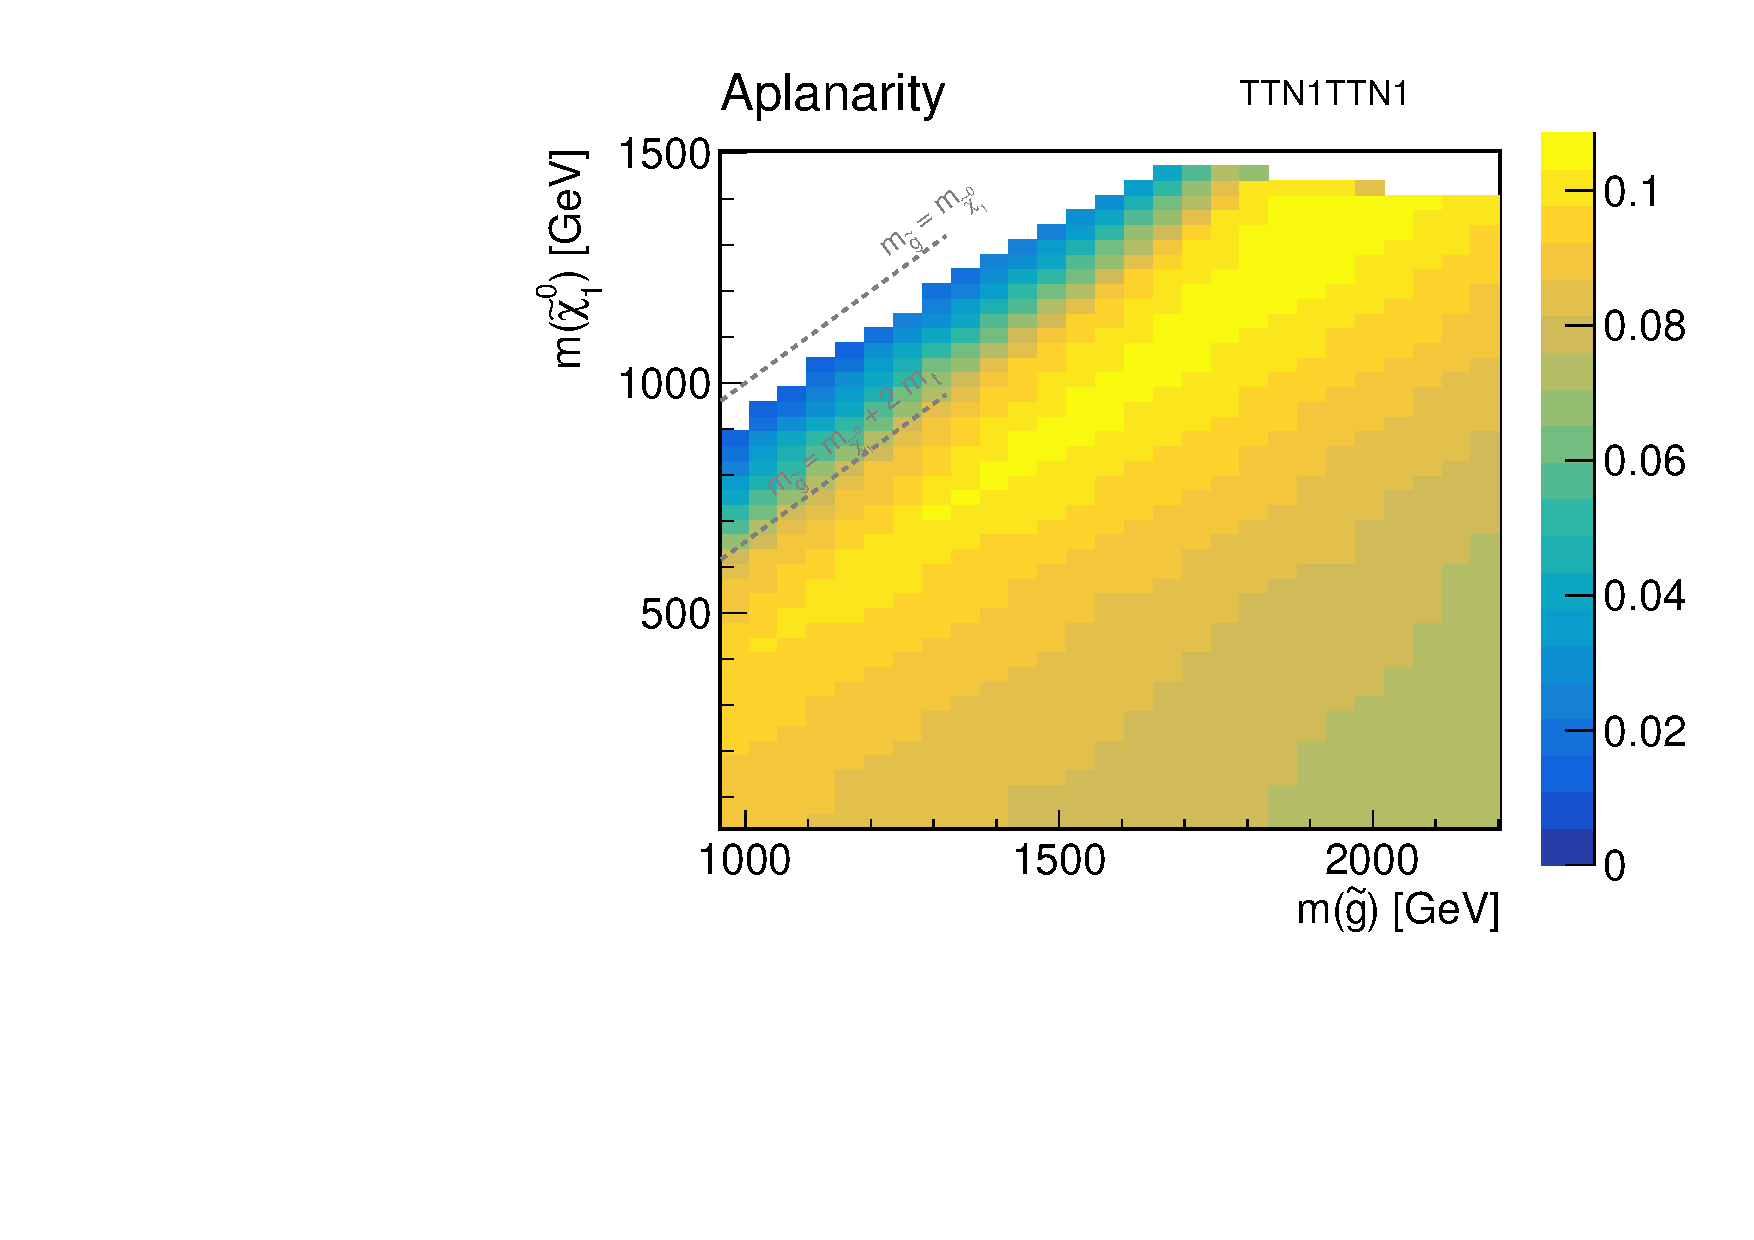
\includegraphics[width=0.32\textwidth]{figures/SRdefinition/kineMap/GG_symTTN1_x12_LepAplanarity.pdf}}
    \subfigure[]{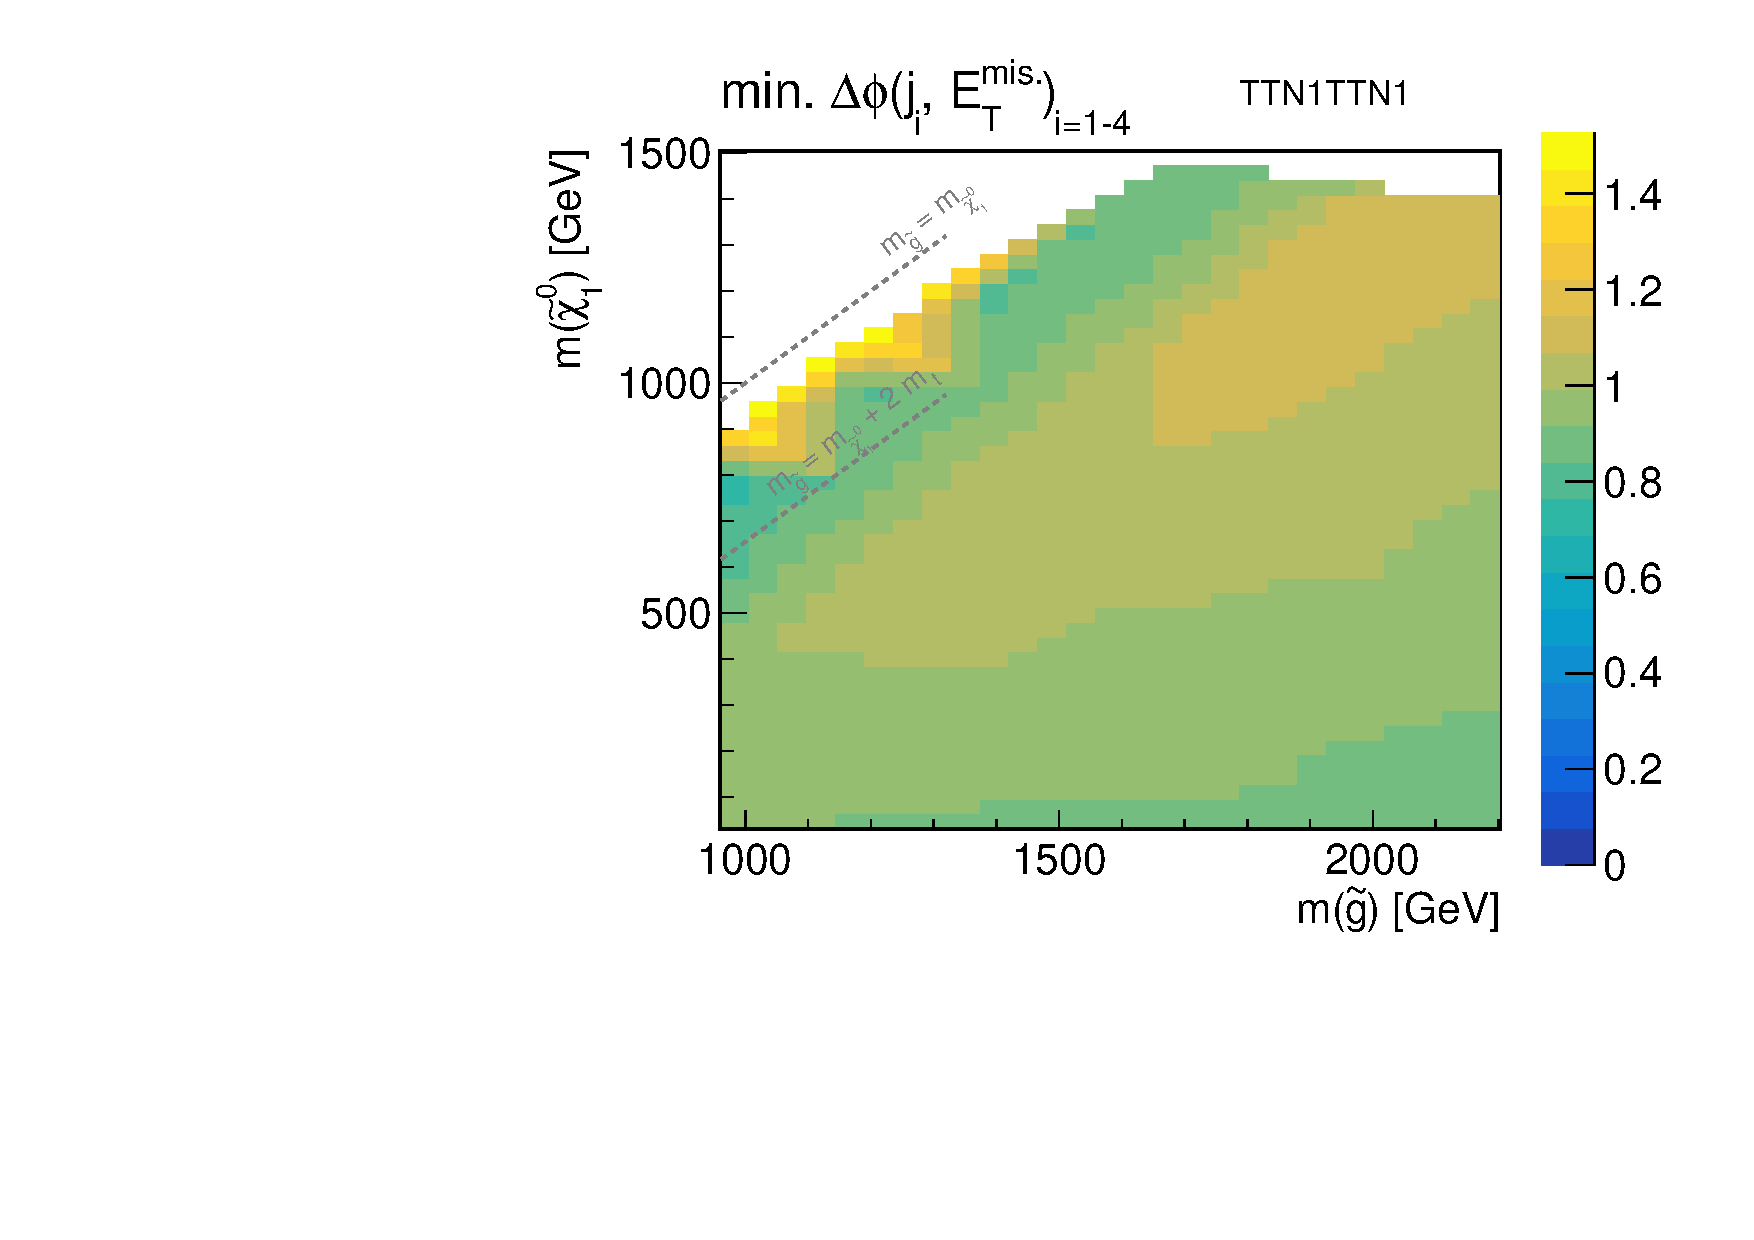
\includegraphics[width=0.32\textwidth]{figures/SRdefinition/kineMap/GG_symTTN1_x12_min_dPhi_4j.pdf}}
    \subfigure[]{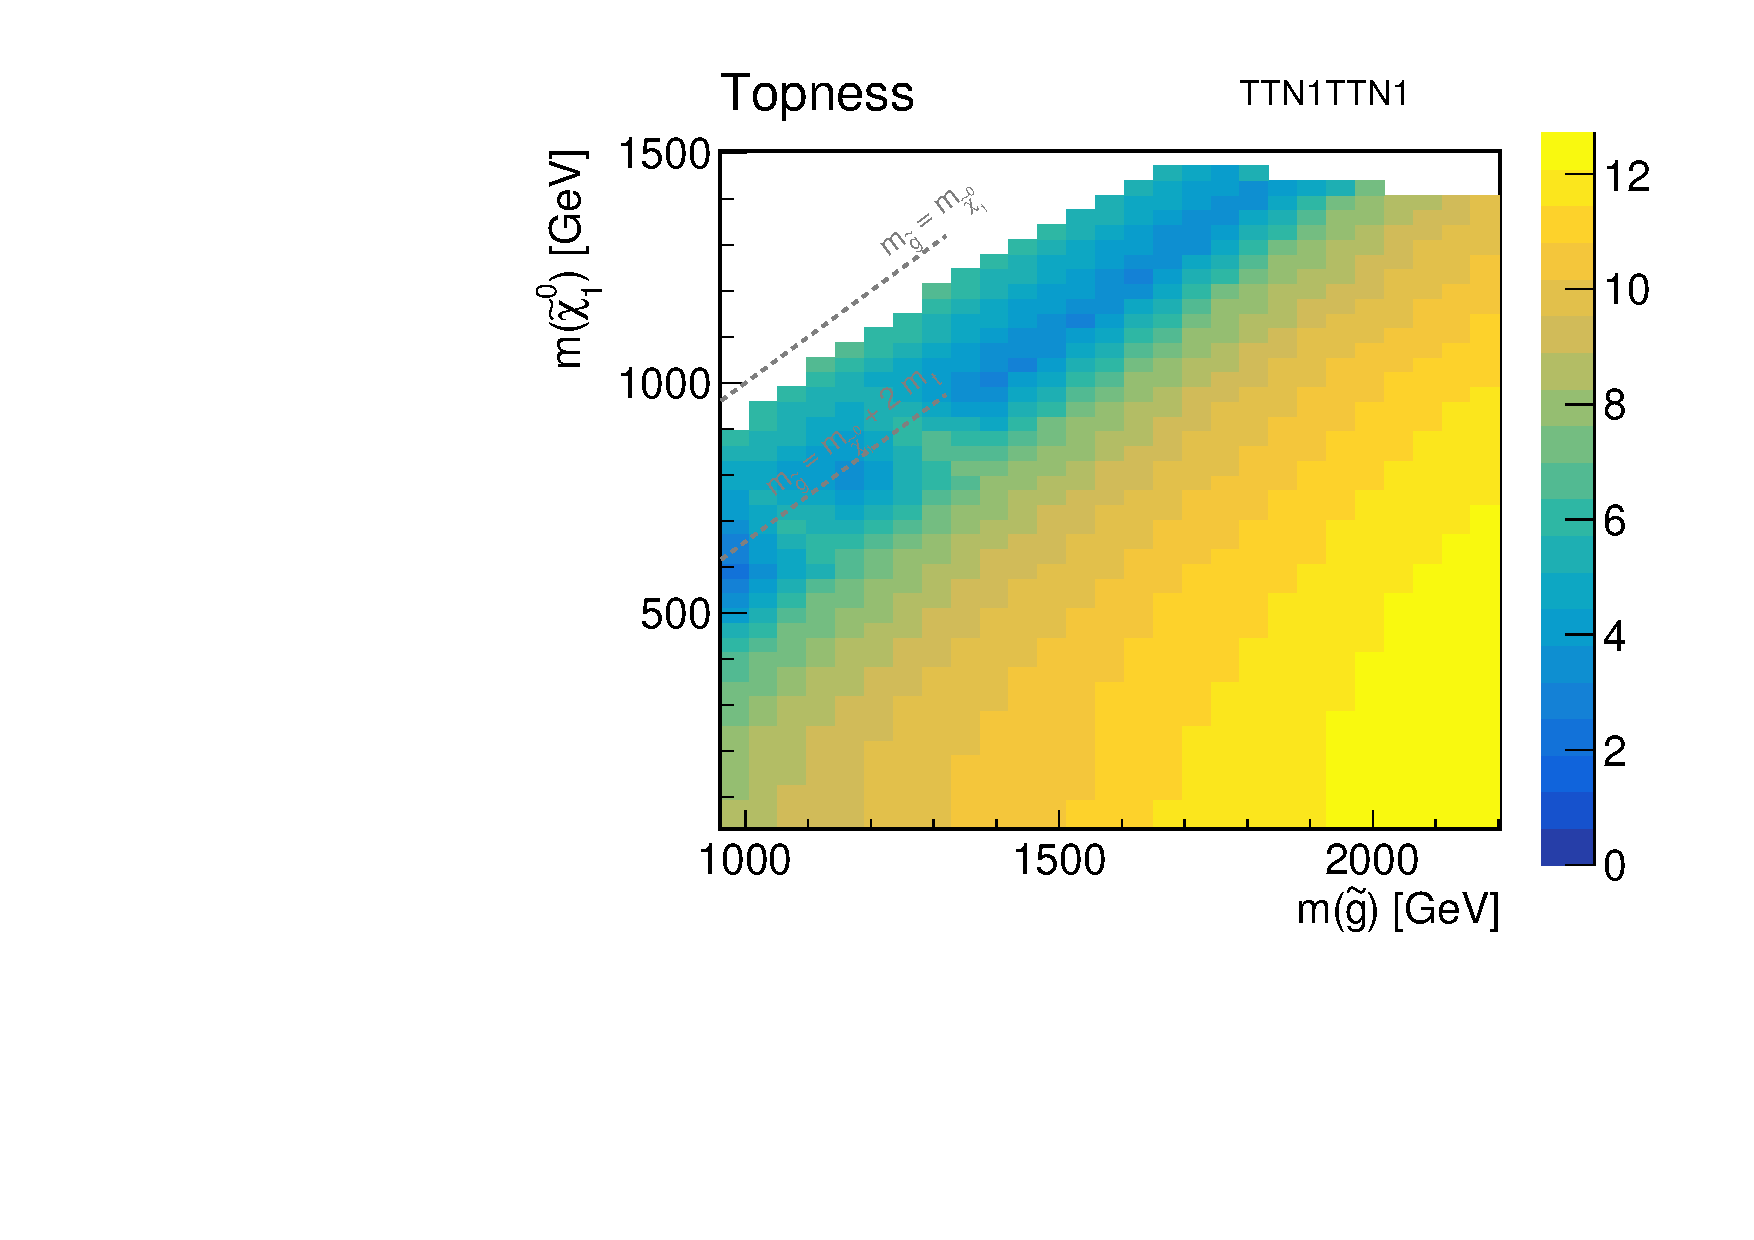
\includegraphics[width=0.32\textwidth]{figures/SRdefinition/kineMap/GG_symTTN1_x12_topNess.pdf}}
    \caption{ Mean of (a) jet-multiplicity ($p_T>30\gev$) (b) bjet-multiplicity ($p_T>30\gev$) (c) $\meffInc$ (d) $\met$ (e) $\lepPt$ (f) $\mt$ (g) aplanarity (h) $\mindPhiFourJet$ (i) topness, for the TTN1TTN1 \dire grid, after the pre-selection. 
      \label{fig::SRdefinition::kineMap_TTN1TTN1} 
    }
\end{figure}
